\documentclass{scrartcl}
\usepackage[utf8]{inputenc}
\usepackage[english]{babel}
\usepackage{caption}
\usepackage{subcaption}
\usepackage{listings}
\usepackage{pdfpages}
\usepackage{amsmath,amssymb}
\usepackage{siunitx}
\usepackage{hyperref}
\usepackage{mhchem}
\usepackage[section]{placeins}
\usepackage[activate, protrusion=true, expansion=true]{microtype}
\usepackage[left=2.5cm, right=2.5cm, bottom=2.5cm, top=2.5cm]{geometry}
\usepackage{libertine}
\usepackage{longtable}
\usepackage{bbm}

\definecolor{mygreen}{rgb}{0,0.6,0}
\definecolor{mymauve}{rgb}{0.58,0,0.82}
\definecolor{mygray}{rgb}{0.5,0.5,0.5}
\lstset{
  backgroundcolor=\color{white},
  keepspaces=true,
  captionpos=b,
  keywordstyle=\color{blue},
  language=matlab,
  stringstyle=\color{mymauve},
  tabsize=2,
  numbers=left,                    % where to put the line-numbers; possible values are (none, left, right)
  numbersep=5pt,                   % how far the line-numbers are from the code
  numberstyle=\tiny\color{mygray},
  basicstyle=\footnotesize,        % the size of the fonts that are used for the code
  breakatwhitespace=false,         % sets if automatic breaks should only happen at whitespace
  breaklines=true,                 % sets automatic line breaking
  commentstyle=\color{mygreen},    % comment style
  deletekeywords={input},            % if you want to delete keywords from the given language
}

\newcommand*{\matlabcode}[3]{\begin{figure}[h!]\lstinputlisting[caption=#2, label=#3]{#1}\end{figure}}

\usepackage{scrpage2}
\pagestyle{scrheadings}
\automark{section}
\ihead{\rightmark}
\chead{}
\ohead{
\includegraphics[scale=0.025]{figures/EPFL_Logo.png}}
\setheadsepline{.4pt}

\begin{document}

%!TEX root = ./exercice2.tex

\begin{titlepage}
	\title{CE-2: Parametric Identification Methods} % Title
	\author{Arne Sachtler \\ Julia Krottenthaler}		% Author
	\date{\today}								% Date

	\makeatletter
	\let\thetitle\@title
	\let\theauthor\@author
	\let\thedate\@date
	\makeatother

	\centering
	\vspace*{0.5 cm}

    
\includegraphics[width=0.7\linewidth]{figures/EPFL_Logo.png}\\[1.0 cm]	
	\textsc{\Large System Identification (ME-421)}\\[1.0cm]				
	\rule{\linewidth}{0.2 mm} \\[0.5 cm]
	{ \LARGE \thetitle}\\
	\rule{\linewidth}{0.2 mm} \\[1.5 cm]
	
    \vspace{1cm}
	\begin{minipage}{0.5\textwidth}
		\begin{flushleft} \large
			\emph{{Students}:}\\
			\theauthor
			\end{flushleft}
			\end{minipage}~
			\begin{minipage}{0.4\textwidth}
			\begin{flushright} \large
			\emph{{Lecturer}:} \\	
			Prof. Karimi Alireza  \\
		\end{flushright}
	\end{minipage}\\[1.2cm]
	{\vspace{3cm} \large Lausanne, \thedate}\\[1.5 cm]
	\vfill
\end{titlepage}

\tableofcontents
%!TEX root = ./exercice2.tex

\section{Identification of a Laser Beam Stabilizing System}
The following section explain identification algorithms using data from the laser beam stabilizing system shown in Figure~\ref{fig:system}.
We have access to time-domain data in the file \texttt{laserbeamdataN.mat}.
This file contains the input $u$ and the output signal $y$ of the laser beam stabilizing system and has $N=500$ samples.

\begin{figure}[h]
	\centering
	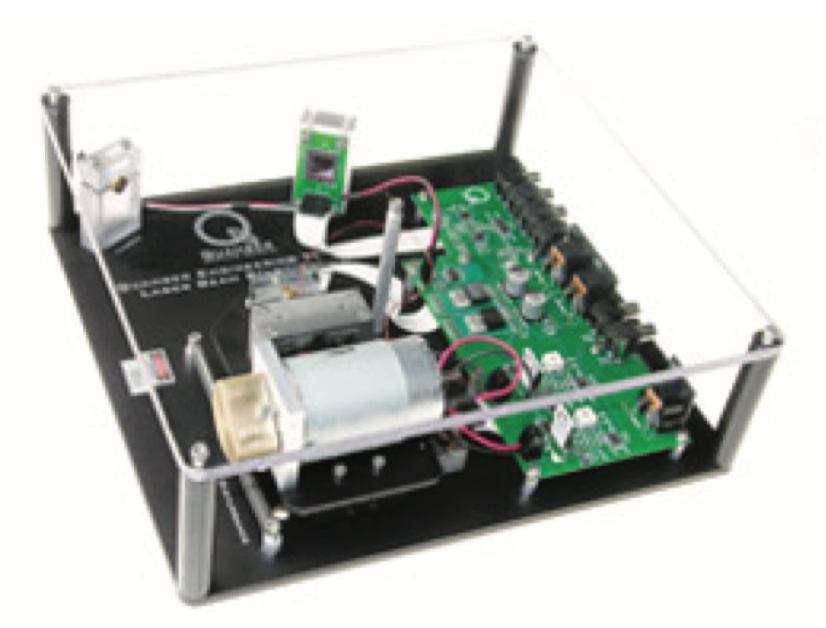
\includegraphics[height=4cm]{figures/system.png}
	\caption{Laser beam stabilizing system }\label{fig:system}
\end{figure}

\subsection{FIR Model Identification}\label{sec:FIR}
In this section we identify a finite impulse response (FIR) model of the form
\begin{equation}\label{eq:FIRmodel}
	\hat{y}(k,\theta) = b_1 u(k-1) + \cdots + b_m u(k-m) \qquad m = 1,2,\ldots,50 \, ,
\end{equation}
which can be rewritten to
\begin{align}\label{eq:FIRrewritten}
	 \hat{y} (k,\theta) & = \phi^{T} (k) \theta 
 \intertext{where}
 	 \phi^{T} (k) & = \left[ u(k-1), u(k-2), \ldots, u(k-m) \right] \\
 	 \theta^T & = \left[ b_1, b_2, \ldots, b_m \right] .
\end{align}

First, we compute the parameter vector $\hat{\theta}$ using the least squares algorithm and the Moore-Penrose pseudo inverse $\pmb{\phi}^+$ of $\pmb{\phi}$
\begin{equation}\label{eq:FIRmodel}
	\hat{\theta} = \left[ \sum\limits_{k=1}^N \phi(k)\phi^T(k) \right]^{-1} \sum\limits_{k=1}^N 
\phi(k) y(k) = \left( \pmb{\phi}^T \pmb{\phi} \right)^{-1} \pmb{\phi}^T \textbf{Y} = \pmb{\phi}^+ \textbf{Y}.
\end{equation}
Here, $\pmb{\phi}$ is an asymmetric (lower) triangular Toeplitz matrix, which we generate with the MATLAB \texttt{toeplitz} command.
In MATLAB we can solve this least squares problem by simply using the backslash operator. 
Afterwards, we compute the predicted output of our identified model $\hat{y} (k,\hat{\theta}) = \phi^{T} (k) \hat{\theta}$. 
The code is shown in Listing~\ref{lst:FIR} (page~\pageref{lst:FIR}) and the result can be seen in Figure~\ref{fig:output_fir}.
\begin{figure}[h]
	\centering
	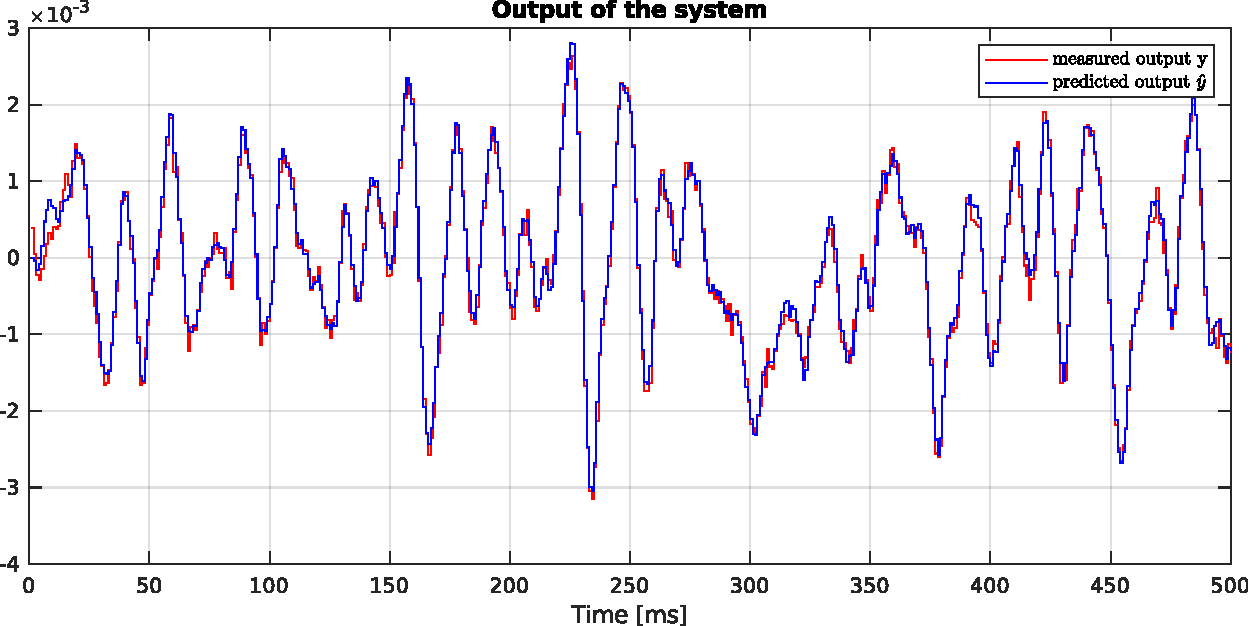
\includegraphics[height=5.5cm]{figures/output.pdf}
	\caption{Predicted and measured output of the system}\label{fig:output_fir}
\end{figure}
In order to estimate the quality of our predictor, we need a fit criterion, which should minimized. We therefore consider the function
\begin{equation}\label{eq:J}
	J(\theta) = \sum\limits_{k=1}^N \left[y(k) - \hat{y}(k,\theta) \right]^2.
\end{equation}
Using the MATLAB command \texttt{norm} and squaring the result we obtain $ J(\theta) \approx 6.92 \cdot 10^{-6}$. 
As we assume that the noise is white, we obtain an unbiased estimate of the noise variance using
\begin{equation}\label{eq:sigma}
	\hat{\sigma}_{noise}^{2} = \frac{1}{N-m} J(\hat{\theta}) .
\end{equation}
Using the available data this equation yields to $ \hat{\sigma}_{noise} \approx 1.24 \cdot 10^{-4} $.
The covariance of the parameter estimates can then be obtained using
\begin{equation}\label{eq:cov}
	cov[\hat{\theta}] = \hat{\sigma}_{noise}^2 \left[ \sum\limits_{k=1}^N \phi(k)\phi^T(k) \right]^{-1} = \hat{\sigma}_{noise}^2 \left( \pmb{\phi}^T \pmb{\phi} \right)^{-1} .
\end{equation}
The square root of the diagonal elements of the $cov[\hat{\theta}]$ matrix is the standard deviation $ \sigma $, which we use for the $ \pm 2 \sigma $ confidence interval in Figure~\ref{fig:fir_response}. This figure shows us the finite impulse response of the system.
\begin{figure}[h]
	\centering
	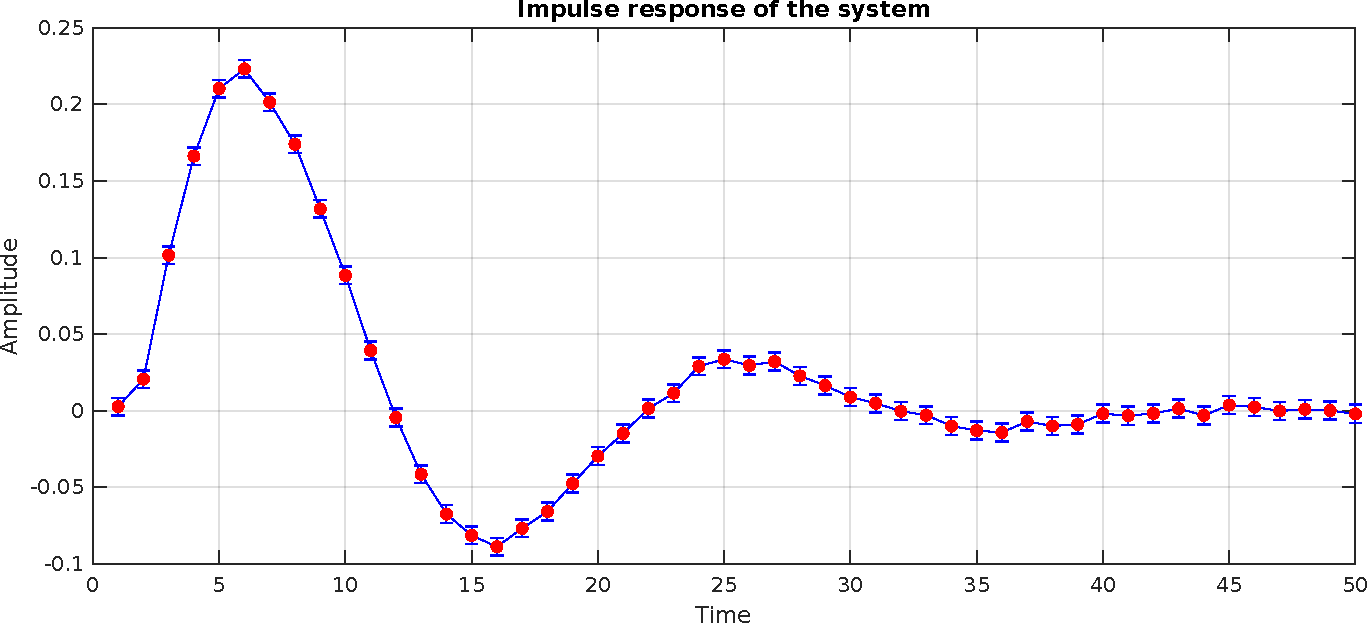
\includegraphics[height=5.5cm]{figures/fir_response.pdf}
	\caption{Identified finite impulse response of the laser beam stabilization system. The error bars show the $2\sigma$ confidence interval of the estimates.}\label{fig:fir_response}
\end{figure}

\subsection{ARX Model Identification}
We now assume a second order auto-regressive with external input (ARX) model for the same data as in the previous section. 
Consequently, we use the following predictor
\begin{align}\label{eq:arx}
	\hat{y}(k,\theta) & = -a_1 y(k-1) - a_2 y(k-2) + b_1 u(k-1) + b_2u (k-2) = \phi^T(k) \theta
	\intertext{where}
 	 \phi^{T} (k) & = \left[ -y(k-1), -y(k-2), u(k-1), u(k-2) \right] \\
 	 \theta^T & = \left[ a_1, a_2, b_1, b_2\right] .
\end{align}
We observe that the system has no modeled delay as $d = 0$.
Using the least squares algorithm and the Moore-Penrose pseudo inverse $\pmb{\phi}^+$ of $\pmb{\phi}$, we compute, like we already did in Section~\ref{sec:FIR}, the parameter vector $\hat{\theta}$ according to
\begin{equation}\label{eq:ARXmodel}
	\hat{\theta} = \left[ \sum\limits_{k=1}^N \phi(k)\phi^T(k) \right]^{-1} \sum\limits_{k=1}^N 
\phi(k) y(k) = \left( \pmb{\phi}^T \pmb{\phi} \right)^{-1} \pmb{\phi}^T \textbf{Y} = \pmb{\phi}^+ \textbf{Y}.
\end{equation}
We construct the matrix consisting of the input and output values according to the predictor structure and solve for the parameters using the backlash operator.
Listing~\ref{lst:ARX} on page~\pageref{lst:ARX} shows the implementation in Matlab.
The predicted output of our identified model $\hat{y}(k,\hat{\theta})$ is then computed using $\hat{y}(k,\hat{\theta}) = \phi^{T} (k) \hat{\theta}$. 
The result can be seen in Figure~\ref{fig:output_arx}.
Note that this predictor (in contrast to the simulated transfer function below) uses the measured past value of the output.
In order to estimate the quality of our predictor, we need a fit criterion, which should minimized. Hence, we consider a loss function as 
\begin{equation}\label{eq:J}
	J(\theta) = \sum\limits_{k=1}^N \left[y(k) - \hat{y}(k,\theta) \right]^2.
\end{equation}
Using this, we obtain $ J(\theta) \approx 2.17 \cdot 10^{-5}$. 
Afterwards we compute the output of the identified model $y_m(k)$ using the MATLAB command \texttt{lsim} and the transfer function of the model
\begin{equation}
	G_0(q) = \frac{b_1 q^{-1} + b_2 q^{-2}}{1 + a_1 q^{-1} + a_2 q^{-2}}
	= \frac{0.0183q^{-1} + 0.0731q^{-2}}{1 - 1.5483q^{-1} + 0.6484q^{-2}}\, .
\end{equation}
We generate a transfer function object using the MATLAB command \texttt{tf} and simulate the output given the input $u(k)$ and we plot the simulated output resulting from the second order model with the measured output in Figure~\ref{fig:output_lsim2}.
The resulting sum of the squares of the error is then $ J_{tf}(\hat{\theta}) \approx 1.14 \cdot 10^{-4}$. 
\begin{figure}[h!]
	\centering
	\begin{subfigure}{.49\textwidth}
		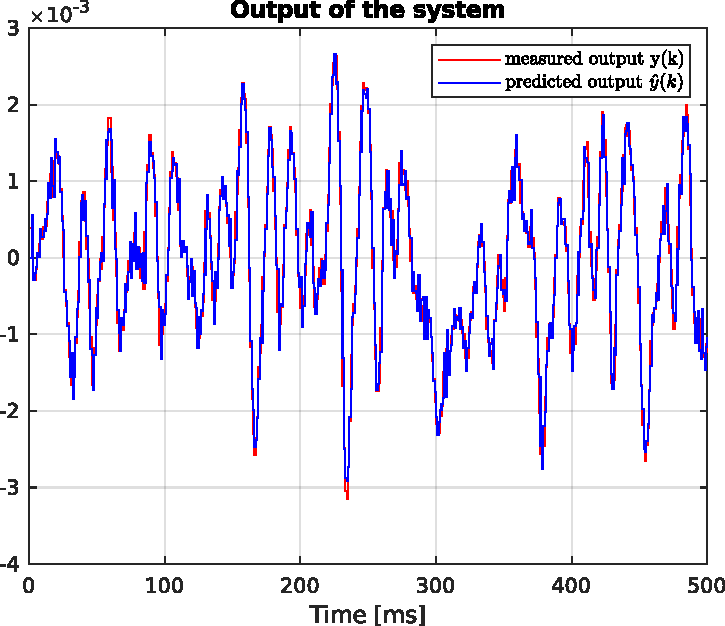
\includegraphics[width=\textwidth]{figures/output_arx.pdf}
		\subcaption{Comparison of measured output $y$ and predicted output $\hat{y}$ using the past measured output.}\label{fig:output_arx}
	\end{subfigure}\hfill
	\begin{subfigure}{.49\textwidth}
		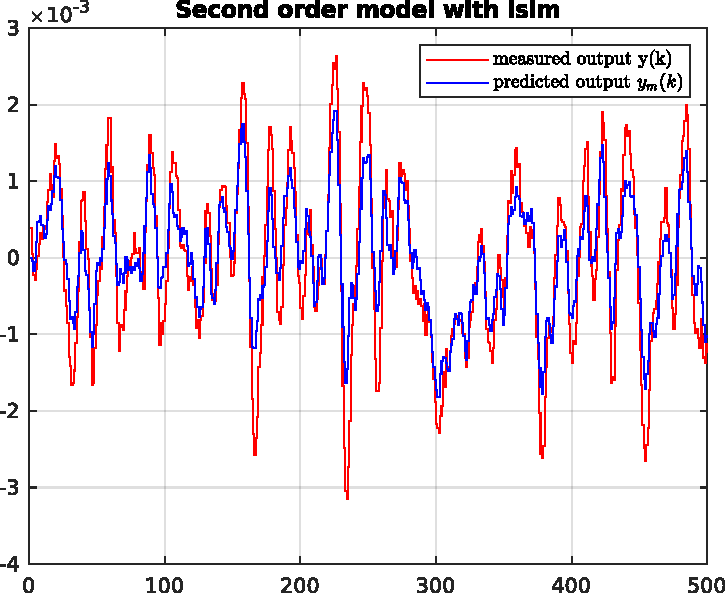
\includegraphics[width=\textwidth]{figures/output_lsim2.pdf}
		\subcaption{Comparison of measured output $y$ and predicted output $y_m$ using only the input and a transfer function model.}\label{fig:output_lsim2}
	\end{subfigure}
	\begin{subfigure}{\textwidth}
		\vspace*{1cm}
		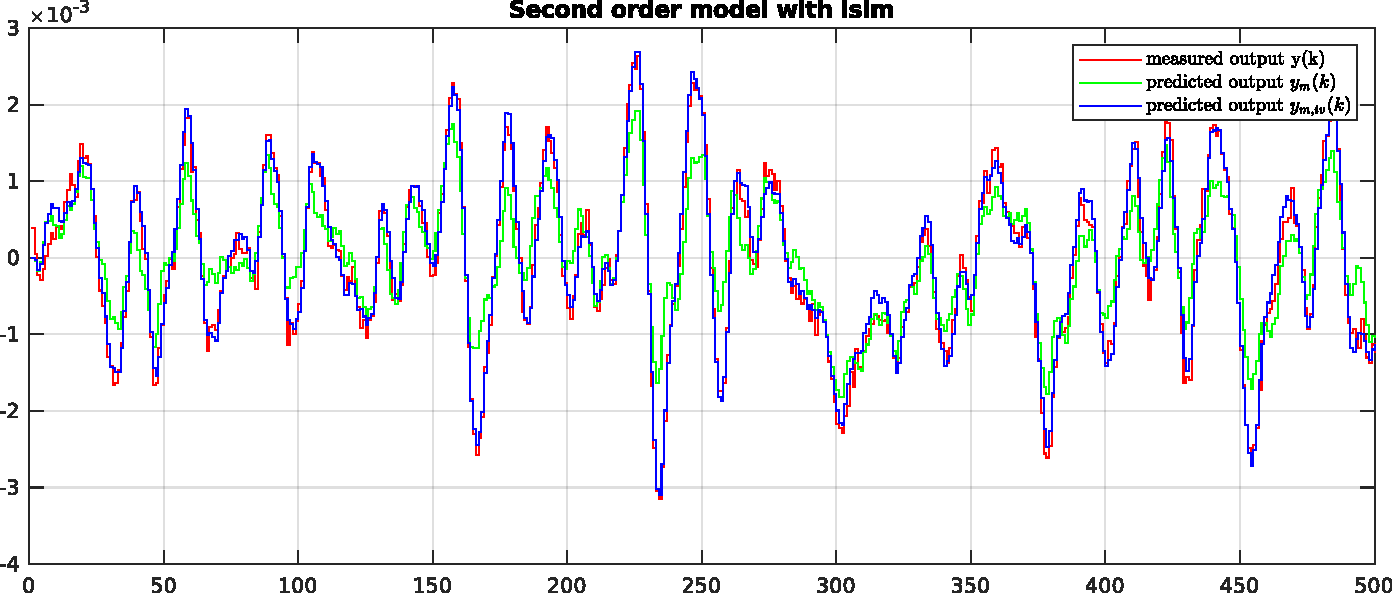
\includegraphics[width=\textwidth]{figures/arx_iv.pdf}
		\subcaption{Comparison of the measured output and the predicted output. The simulated output is shown for the model parametrized by the parameters identified using the plain ARX method and the IV method with $4$ iterations, respectively.} \label{fig:output_arx_iv}
	\end{subfigure}
	\caption{Comparison of predicted and measured output. Upper part: comparison with predictor using the past measured output and comparison only using the input data and the simulated transfer function model. Lower part:comparison of ARX model with IV method and past measured output}
\end{figure}
In order to obtain unbiased estimates the following two conditions must be satisfied: 
\begin{enumerate}
\item $R_{\phi \phi}$ is not singular,
\item $R_{\phi e }(0) = 0$.
\end{enumerate}
These conditions can be satisfied by replacing the non-transposed $\phi$'s in the estimator for $\hat{\theta}$ by a new vector $\phi_{iv}$ called the vector of  instrumental variables (IV):
\begin{equation}
	\hat{\theta}_{iv} = \left[ \sum\limits_{k=1}^N \phi_{iv}(k)\phi^T(k) \right]^{-1} \left[\sum\limits_{k=1}^N \phi_{iv}(k) y(k) \right]
\end{equation}
Therefore, the estimates are asymptotically unbiased, if 
\begin{enumerate}
	\item $R_{\phi_{iv} \phi}$ is not singular,
	\item $R_{\phi_{iv} e }(0) = 0$.
\end{enumerate}
That means, choosing an vector of instrumental variables, that is correlated with the regressor vector $\phi$ and uncorrelated with the noise $e$ leads to asymptotically unbiased estimates.
One choice of this vector is keeping the past, non-noisy inputs in the vector and replacing the past noisy outputs using the output of an already identified model $M(q^{-1})$. A noiseless output of this model can be computed by 
\begin{equation}
y_m(k) = M(q^{-1}) u(k)
\end{equation}
and the vector $\phi_{iv}$ is defined as
\begin{equation}
\phi_{iv}^T(k) = \left[-y_M(k-1),\ldots,-y_M(k-n),u(k-d-1),\ldots,u(k-d-m)\right]
\end{equation}
with $d=0$. 
Therefore, we can first identify an ARX model without the use of instrumental variables. 
Afterwards, we use the identified parameters as instrumental variables and repeat the ARX fitting.
In order to obtain better results, this process can be repeated for several iterations. 
For a good trade off between computational cost and accuracy, we choose an IV method with $4$ iterations. 
The result of the instrumental variables method compared to the measured output and the predicted output of the transfer function model can be seen in Figure~\ref{fig:output_arx_iv} and the implementation can be viewed, again, in Listing~\ref{lst:ARX} (page~\pageref{lst:ARX}).
Note that the function performs ARX identification with and without the IV method.
Setting \texttt{iterations} to 1 means that no IV method is used.
We can observe, that the predicted output of the model identified using the IV method is closer to the measured output.

\subsection{State-space Model Identification}
In this part, a state-space model for the laser beam stabilizing system using the subspace method based on the extended observability matrix is identified. \\
First, the following matrices are defined: 
\begin{align}
 Y &= \left[Y_r(1), Y_r(2),\ldots,Y_r(N) \right] \\
 U &= \left[U_r(1), U_r(2),\ldots,U_r(N) \right] \\
 X &= \left[x_r(1), x_r(2),\ldots,x_r(N) \right]
\end{align}
with 
\quad $Y_r(k) = \left[ \begin{array}{c} y(k) \\\ y(k+1) \\\ \vdots \\\ y(k + r -1) \end{array}\right] $ , \quad $U_r(k) = \left[ \begin{array}{c} u(k) \\\ u(k+1) \\\ \vdots \\\ u(k + r -1) \end{array}\right] $ \quad and \quad $r > n $\\
The output of the noise-free state-space model can be written as
\begin{equation}
y(k+i) = CA^{i}x(k) + CA^{i-1}Bu(k) + CA^{i-2}Bu(k+1) + \cdots + CBu(k+i-1) + Du(k+i)
\end{equation}
and as 
\begin{equation}
\textbf{Y} = O_r \textbf{X} + S_r \textbf{U}
\label{eq:statespace}
\end{equation}
respectively. 
To get rid of the unknown matrix $S_r$ the following $ N \times N $ matrix is formed: 
\begin{equation}
\textbf{U}^{\bot} = \textbf{I} - \textbf{U}^{T}(\textbf{U}\textbf{U}^{T})^{-1}\textbf{U} \quad \text{with} \quad \textbf{U}\textbf{U}^{\bot} = 0.
\end{equation}
By multiplying Equation~\ref{eq:statespace} with $\textbf{U}^{\bot}$ from the right, we obtain:
\begin{equation}
	Q = \textbf{Y}\textbf{U}^{\bot} = O_r\textbf{X}\textbf{U}^{\bot}.
\end{equation}
Afterwards, we compute the singular values of $Q$ with the MATLAB command \texttt{svd}. 
Using the singular values of the matrix, we determine the model order by choosing the smallest $n \le r$ such that
\begin{equation}
	\sum\limits_{k=0}^{n}\sigma_k \ge 0.8\sum\limits_{k=0}^{r}\sigma_k\, ,
\end{equation}
i.e. we select the smallest model order $n$ such that the first $n$ singular values sum up to at least $0.8$ of the total sum of the singular values.
Here, we get a model order of $n = 3$.
Then, based on the model order, the matrices for the states space model are computed as provided in the course notes.
The code is shown in Listing~\ref{lst:ss_id} (page~\pageref{lst:ss_id}).
We get the following solutions
\begin{eqnarray}
	\mathbf{A} &=& \begin{bmatrix}
			-0.0645  & 0.0415 & -0.5397\\
			 0.7140  & 0.2319 &  0.1857\\
			-0.3840  & 1.2511 &  0.8986\\
	\end{bmatrix}\,,\\
	\mathbf{B} &=& \begin{bmatrix}
		 -41.5124\\
		-165.7229\\
		-105.1717\\
	\end{bmatrix}\,,\\
	\mathbf{C} &=& 10^{-3} \cdot \begin{bmatrix}
	    0.3697 & -0.0396 & -0.2972
	\end{bmatrix}\, ,\\
	\mathbf{D} &=& 0\, .
\end{eqnarray}

Figure~\ref{fig:ss_id_results} shows the results of the simulation of the identified state-space model using the input data $u$.
We get a residual loss of $J(\theta) = 8.23 \cdot 10^{-6}$.

\begin{figure}[h]
	\begin{subfigure}{0.49\textwidth}
		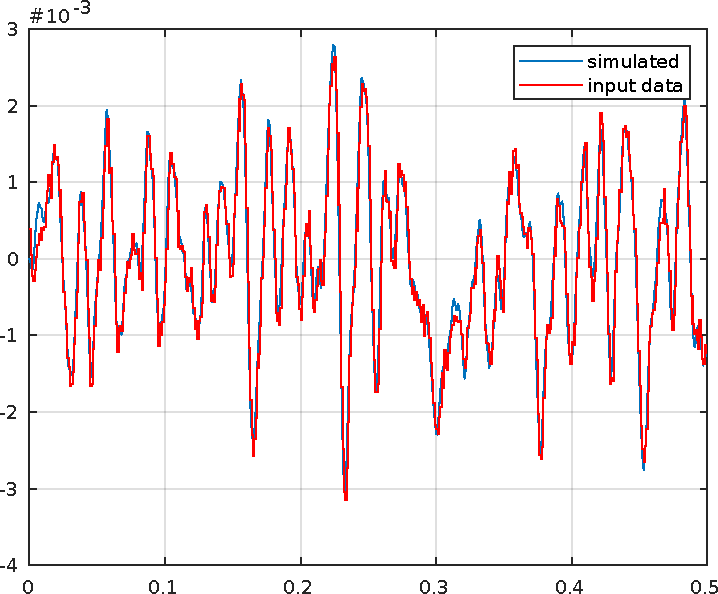
\includegraphics[width=\textwidth]{figures/ss_id_output.pdf}	
		\subcaption{Comparison of outputs}
	\end{subfigure}
	\begin{subfigure}{0.49\textwidth}
		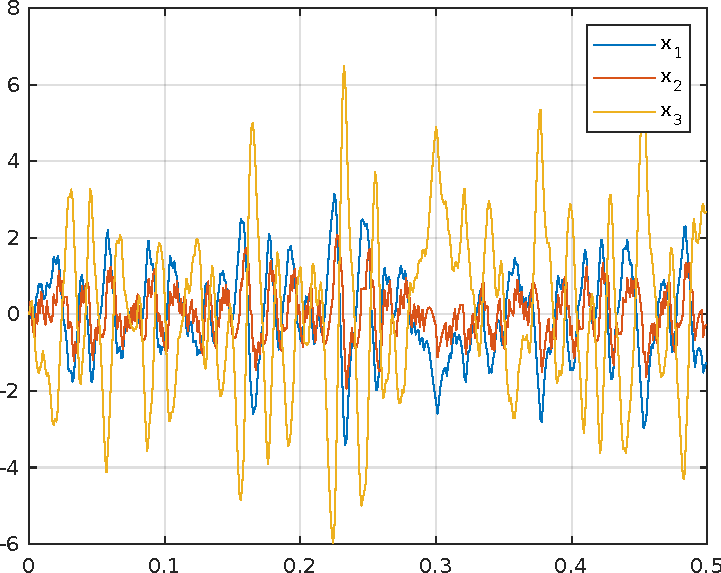
\includegraphics[width=\textwidth]{figures/ss_id_states.pdf}	
		\subcaption{States}
	\end{subfigure}
	\caption{Simulation on the identified state-space model using the input data $u$. On the left the predicted output is compared to the measured output and on the right the evolution of state variable is shown.}
	\label{fig:ss_id_results}
\end{figure}

%!TEX root = ./exercice2.tex

\section{Parametric Identification of an Active Suspension System}
In this section we identify a model between the current reference for the DC motor and the acceleration of the sprung mass of the active suspension system in Figure~\ref{fig:active_suspension}. 
Therefore, we use the time-domain data CE2.mat. This file contains the input $u$ and the output signal $y$ of the system with a set of $N = 2044$ data and a sampling time of $T_e = 0.03$. 
\begin{figure}[h]
	\centering
	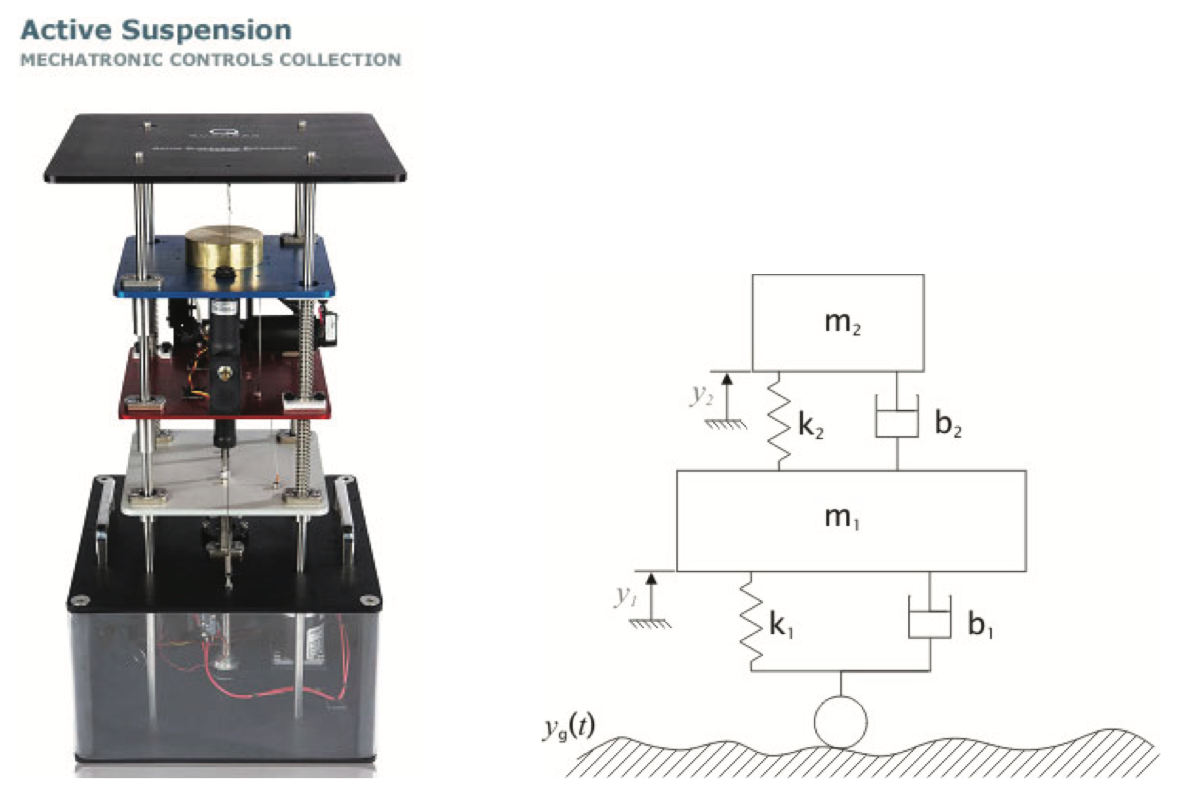
\includegraphics[height=5.5cm]{figures/active_suspension.png}
	\caption{An active suspension system}\label{fig:active_suspension}
\end{figure}
Before we start with the identification procedure, we remove the mean value of the input and output with the MATLAB \texttt{detrend} command and generate a data object with the MATLAB \texttt{iddata}.

\subsection{Order Estimation}
It is one of the goals of system identification to find the simplest model, which meets the desired criteria. Therefore, the model order estimation plays an important role in the procedure. In this section, we focus on finding the order for the Active Suspension System. 

\paragraph{Loss function criterion:} In the first approach, we use the ARX structure. As the loss function $ J(\hat{\theta}) /N $ for this structure is monotonically non-increasing with respect to the number of the parameter estimates (dimension of $\theta$), the model order can be estimated by analyzing the shape of the loss function. We set the delay to $n_k = 0$, the order of the nominator of the plant model $n_b$ equal to the order of the denominator $n_a$ and choose a maximum order of $n=10$. In doing so, we obtain $10$ different ARX models. The corresponding loss function is shown in Figure~\ref{fig:loss_fcn}. 
As the slope of the loss function is close to zero for $n \geq 6 $ we choose a model order equal to $n = 6.$

\begin{figure}[h]
	\centering
	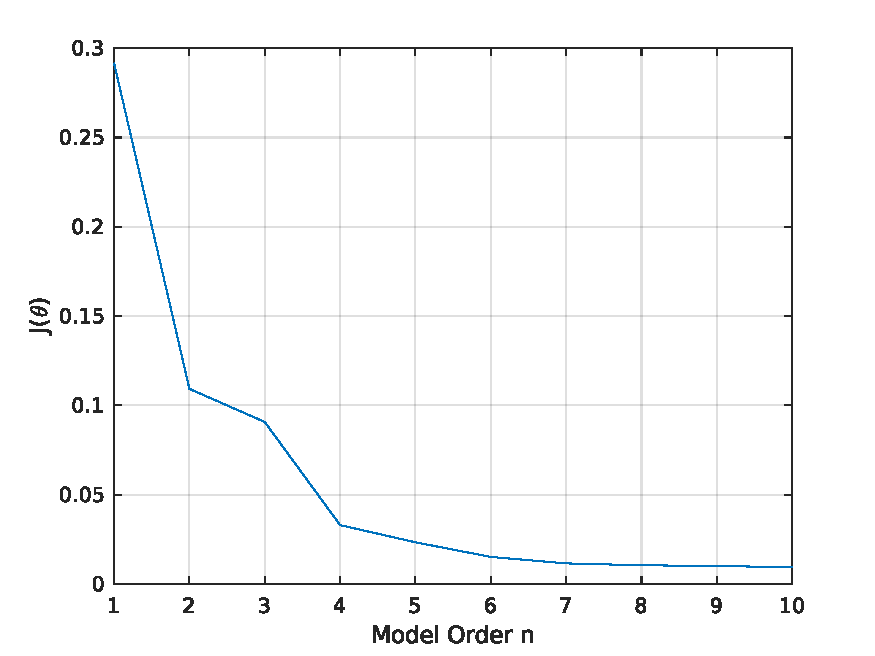
\includegraphics[height=5cm]{figures/Loss_fcn.pdf}
	\caption{Residual losses for different ARX models with varying model order}\label{fig:loss_fcn}
\end{figure}

\paragraph{Zero/Pole cancellation criterion:} Afterwards we want to validate the chosen order by using the zero/pole cancellation method applied to the ARMAX structure for different models. 
We set the order of the plant model $n_a$ and $n_b$ and the order of the noise model $n_c$ to the same value, that means $n_a = n_b = n_c = n $ and the delay equal to one, $n_k = 1$. 
As the estimated order is $6$ according to the loss function method, we choose $ n_{min} \leq n \leq n_{max}$ with $ n_{min} = 5$ and $n_{max}=8$. With the MATLAB command \texttt{iopzplot} we plot the zero/pole map of this $4$ different models, which can be seen in Figure~\ref{fig:zero_pole}. 
As we use noisy data for our identification, an exact zero pole cancellation is impossible (that means an exact overlap between a zero 'o' and a cross 'x' in the map respectively). To solve this issue, a confidence interval with a size of two times their standard deviation $\pm 2 \sigma$ for each pole and zero is plotted. At that point, one zero/pole cancellation indicates, that the order of the model is overestimated by one. 

\begin{figure}[h]
	\centering
	\begin{subfigure}{.49\textwidth}
		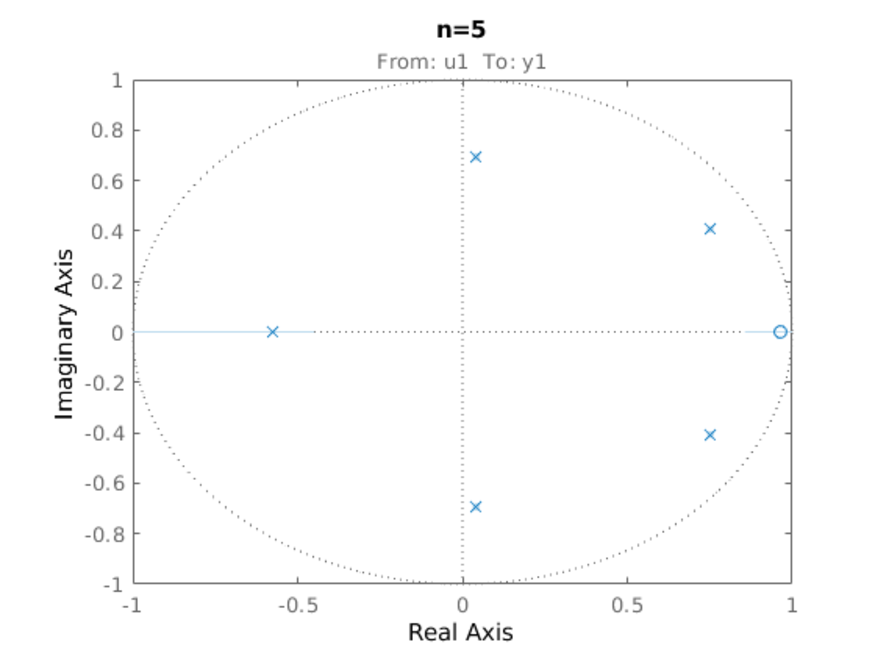
\includegraphics[height=6.5cm]{figures/zp5.pdf}
		\subcaption{Zero/pole map for $n_a = n_b = n_c = 5 $}\label{fig:zp5}
	\end{subfigure}\hfill
	\begin{subfigure}{.49\textwidth}
		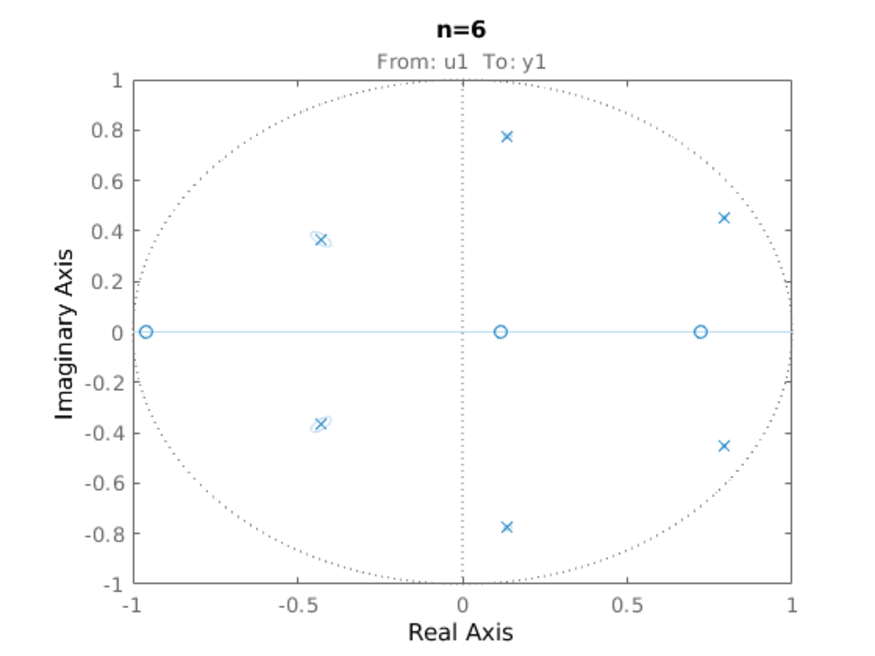
\includegraphics[height=6.5cm]{figures/zp6.pdf}
		\subcaption{Zero/pole map for $n_a = n_b = n_c = 6 $}\label{fig:zp6}
	\end{subfigure}
	\begin{subfigure}{.49\textwidth}
		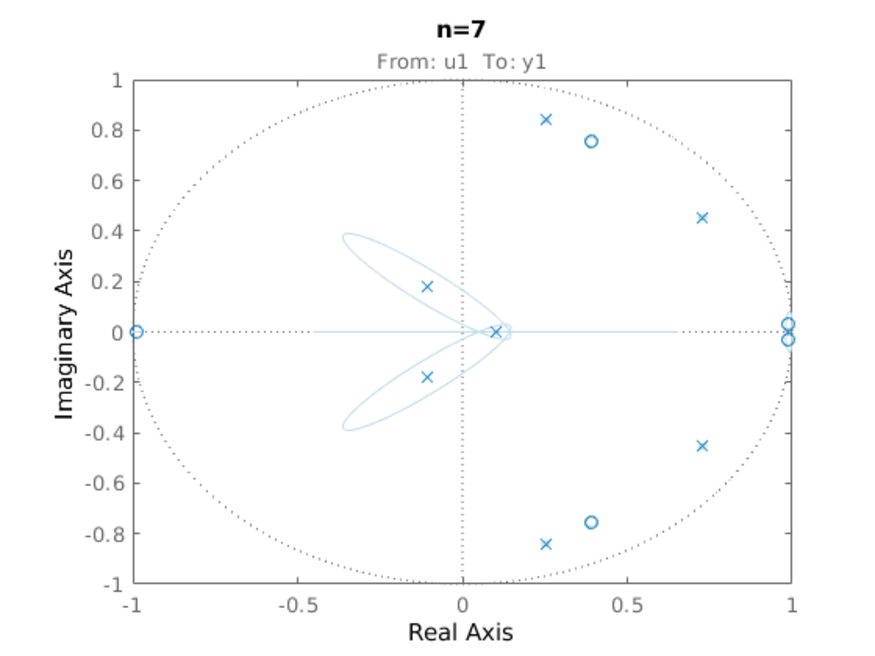
\includegraphics[height=6.5cm]{figures/zp7.pdf}
		\subcaption{Zero/pole map for $n_a = n_b = n_c = 7 $}\label{fig:zp7}
	\end{subfigure}\hfill
	\begin{subfigure}{.49\textwidth}
		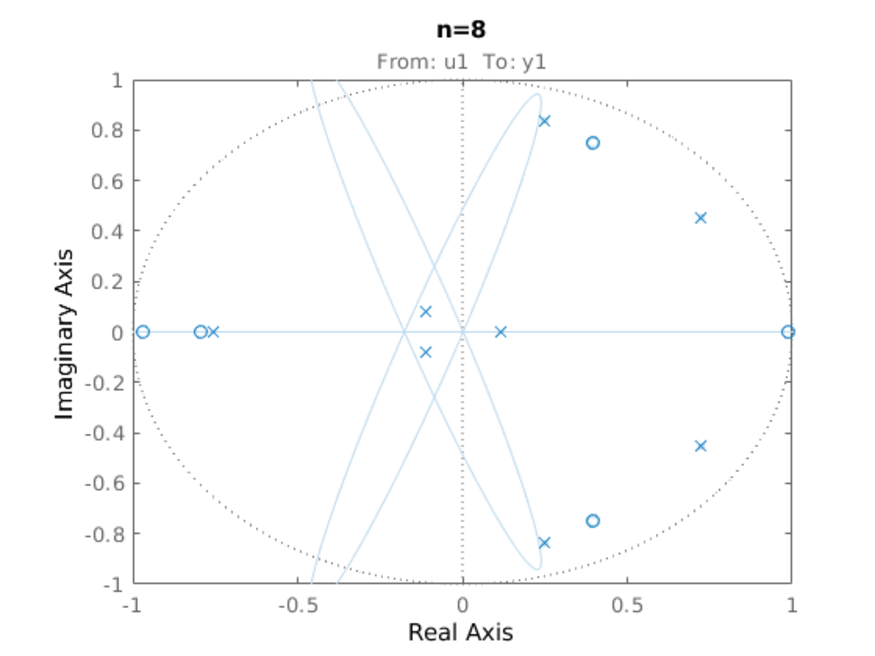
\includegraphics[height=6.5cm]{figures/zp8.pdf}
		\subcaption{Zero/pole map for $n_a = n_b = n_c = 8 $}\label{fig:zp8}
	\end{subfigure}
	\caption{Zero/pole map for different ARMAX models}
	\label{fig:zero_pole}
\end{figure}

The zero/pole cancellation method validates our chosen order $n=6$. For an order of $n=7$ the confidence intervals are significantly larger than for lower orders. That is why we cannot determine the exact value of the poles. \\

\paragraph{Delay estimation:} As a next step, the delay $n_k$ is estimated. This is done by inspecting the impulse response of the system. As the impulse response is equal to the parameters $b_k$ of a FIR model, we use a high order FIR model to plot it. All we have to consider is that the number of parameters $m$ of this model is bigger then the settling time of the impulse response $g(t)$. As $g(t)$ is approximately zero after $ 1 s$ we set the model order to $m = 40$ due to the sampling time $T_e = 0.03 s$.
The time delay $d$ of the system can then be obtained as the number of the first values of the impulse response, that is the first parameters of the FIR model, that are equal to zero. 
However, using noisy data none of the values will be equal to zero. In this case a value can be considered as zero, if $ 0 \in \left[b_k -2 \sigma_k, b_k + 2\sigma_k \right] $ with $\sigma_k$ as the standard deviation of the k-th component. 

In MATLAB, we create the FIR model with the command \texttt{oe}. The code can be seen in Listing~\ref{lst:delay} (page~\pageref{lst:delay}).
Figure~\ref{fig:fir40} shows the impulse response and Figure~\ref{fig:fir40_dev} the parameters with their corresponding confidence interval. As the second value of the impulse response is approximately zero, we estimate the delay as $d=1$ and obtain $n_k = d + 1 = 2$. 

\begin{figure}[h]
	\centering
	\begin{subfigure}{.49\textwidth}
		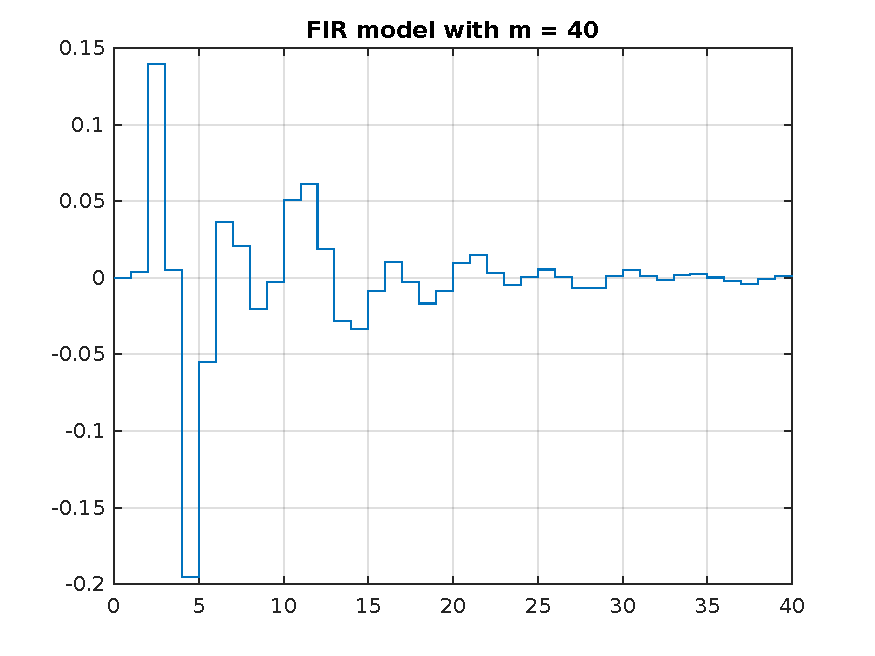
\includegraphics[width=\textwidth]{figures/fir40.pdf}
		\subcaption{Impulse response}\label{fig:fir40}
	\end{subfigure}\hfill
	\begin{subfigure}{.49\textwidth}
		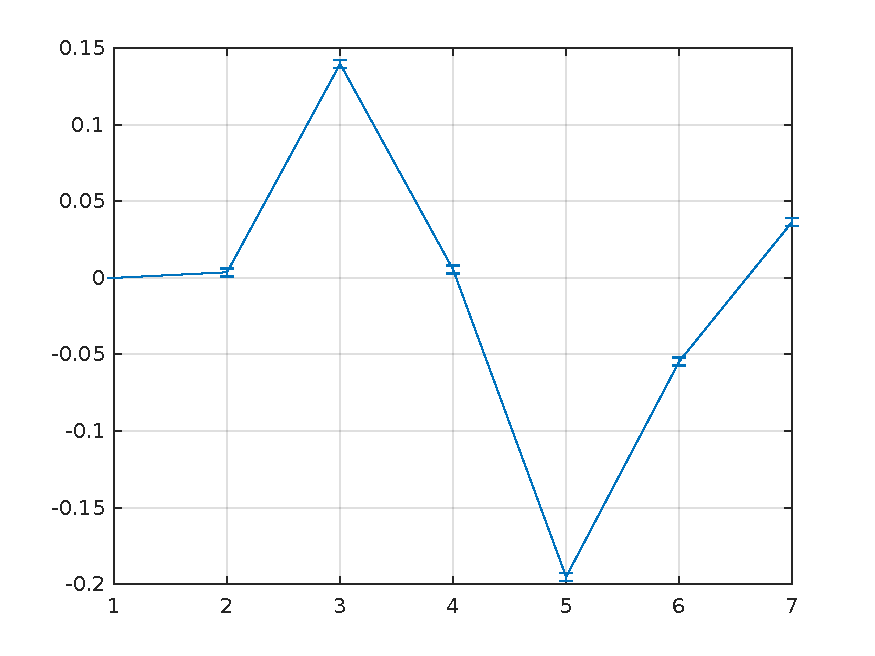
\includegraphics[width=\textwidth]{figures/fir40_dev.pdf}
		\subcaption{Impulse response (zoomed) + confidence interval}\label{fig:fir40_dev}
	\end{subfigure}
	\caption{Impulse response of the system identified using a FIR model and the OE structure. It can be observed, that the second value is nearly equal to $0$. This implies a delay of $1$.}
	\label{fig:delay}
\end{figure}
As the last step, the number of the parameters in the numerator $n_b$ is estimated. This is done by comparing the loss function of different ARX models with a value of $n_b$ as follows: $1 \leq n_b \leq n  - n_k + 1 = 6 - 2 + 1 = 5$. This is done with the MATLAB variable \texttt{M.EstimationInfo.LossFcn}. The results can be seen in Table~\ref{tab:denom}.
As there is only a small reduction of the loss function between $n_b = 5$ and $n_b = 4$ compared to the other steps, we decide to choose $n_b = 4$. \\
Summarized, our estimated parameter values are $n_k = 2$, $n_a = 6$ and  $n_b = 4$.


\begin{table}[h]
	\centering
	\begin{tabular}{l|c}
	\hline
	\hline
	\textbf{Number of parameters $n_b$} & \textbf{Loss function of ARX model}\\
	\hline
		$5$ & $0.0153$ \\ \hline
		$4$ & $0.0161$ \\ \hline
		$3$ & $0.0204$ \\ \hline
		$2$ & $0.0529$ \\ \hline
		$1$ & $0.0711$ \\ \hline
	\hline
	\end{tabular}
	\caption{Loss function for different numbers of parameter in the denominator}
	\label{tab:denom}
\end{table}

\begin{figure}[h]
	\centering
	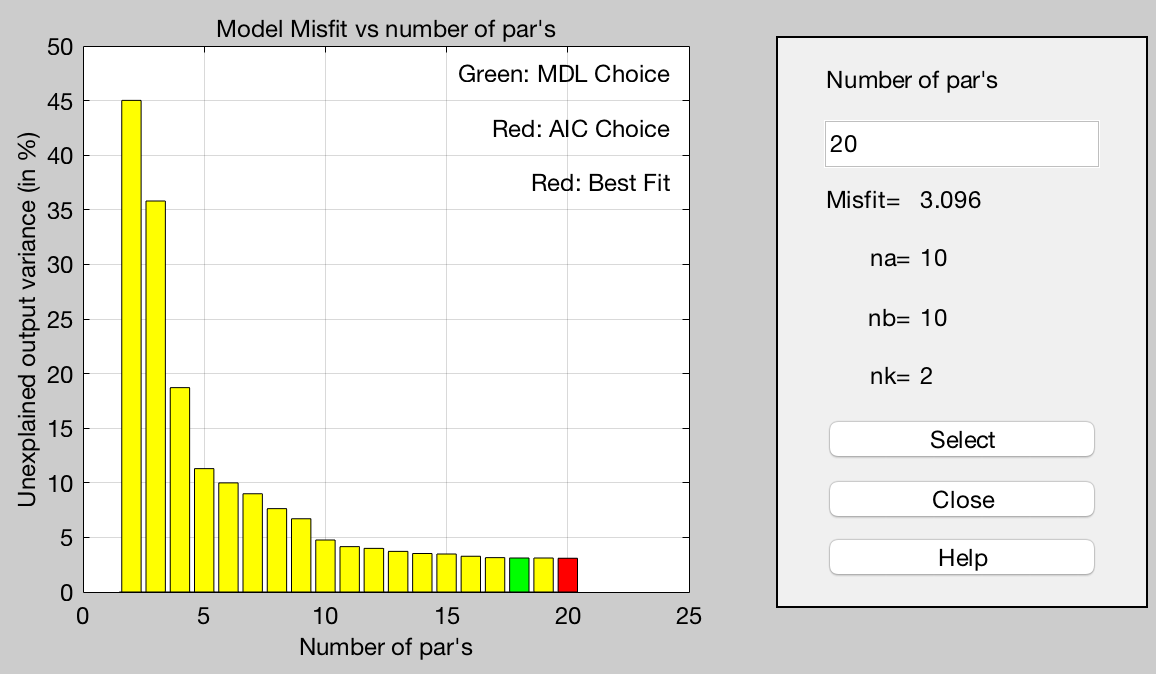
\includegraphics[height=6cm]{figures/selstruc.png}
	\caption{Loss functions calculated with \texttt{arxstruc}}\label{fig:selstruc}
\end{figure}

\paragraph{Comparison to model orders MATLAB proposes:} Finally, we compare our results with those proposed by MATLAB with the commands \texttt{struc}, \texttt{arxstruc} and \texttt{selstruc}. 
With \texttt{struc} we generate $1000$ model-order combinations for the ARX model estimation ($n_a = n_b = n_k = 10)$. Afterwards the loss functions for all the ARX models are calculated with \texttt{arxstruc}. \texttt{selstruc} then allows us to select a model order by showing the values of the different loss functions graphically (Figure~\ref{fig:selstruc}). 
The order proposed by MATLAB via \texttt{struc}, \texttt{arxstruc} and \texttt{selstruc} is significantly larger ($n > 10$). 
This is due to the fact, that MATLAB tries to fit the noise as well and not just only the real data. 
It can be seen in Figure~\ref{fig:selstruc} that the output variance is almost constant for more than $10$ parameters.
As we want a good trade-off between computational cost and the variance, $10$ parameters seems to be a reasonable choice.
This coincides with the choice we made before, since $n_a + n_b = 6 + 4 = 10$. 

\subsection{Parametric Identification}
In this section, we want to create different parametric models using the estimated values for the parameters $n_a$, $n_b$ and $n_k$ from the previous section. 
Therefore, we use various MATLAB commands. 
We create an ARX model, an Instrumental variables method model, an ARMAX model, an Output error structure model, a Box-Jenkins model and a State space models.
Doing that, we divide the data into different parts. 
The first one we use for the model identification and the second one for the model validation. 
Our code for data partitioning and identification with different methods can be viewed in Listing~\ref{lst:parametric} on page~\pageref{lst:parametric}.

\subsection{Model Validation}

\paragraph{Time-Domain Validation:}
As a final step, we want to validate the identified parametric models. Therefore, the data set of $N = 2044$ is again partitioned in two parts. 
The second half of the data, that has not been used for the identification, is used to validate the models. 
First, we compare the output of the models with the measured output of the second half of the data.  
Thereby, the same input is applied to the model and the system. 
The results can be seen in Figure~\ref{fig:comparison}
According to this, the best model is the State Space Model with a fit of $74.98 \% $.

\begin{figure}[h]
	\centering
	\begin{subfigure}{.49\textwidth}
		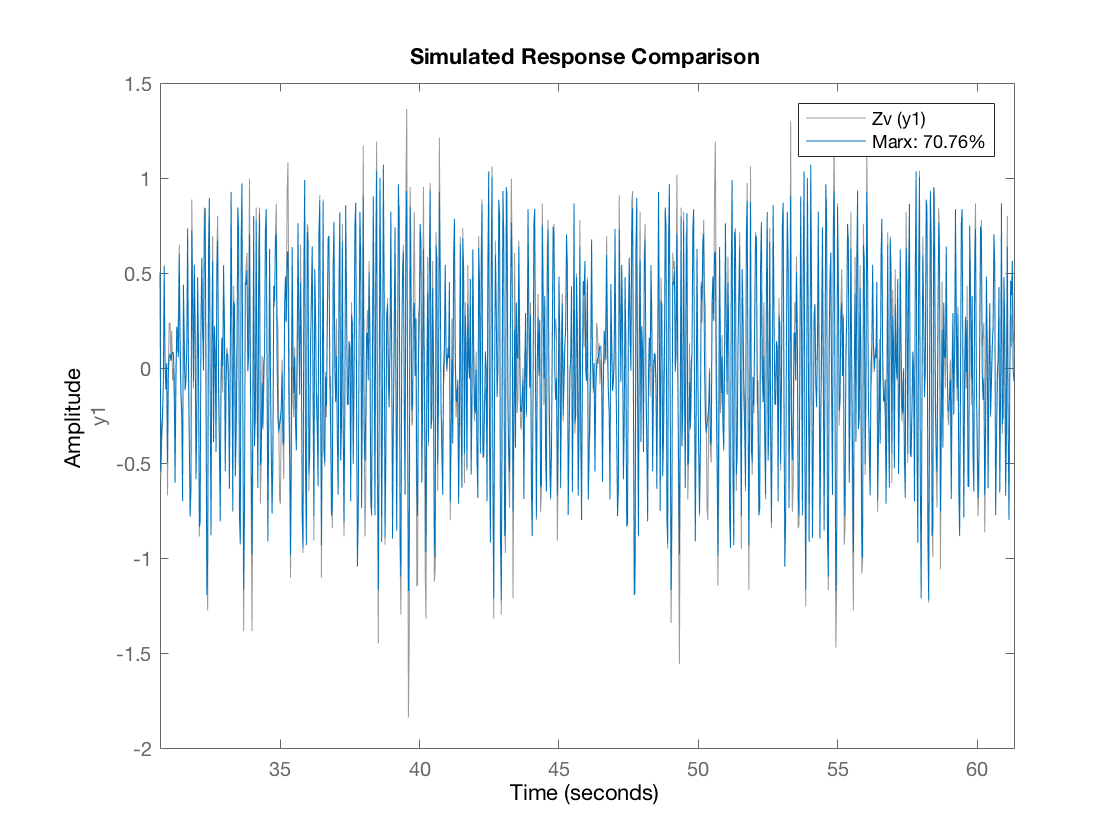
\includegraphics[height=5.5cm]{figures/c_arx.png}
		\subcaption{Comparison of the output of the ARX model with the validation data $Zv$}\label{fig:c_arx}
	\end{subfigure}\hfill
	\begin{subfigure}{.49\textwidth}
		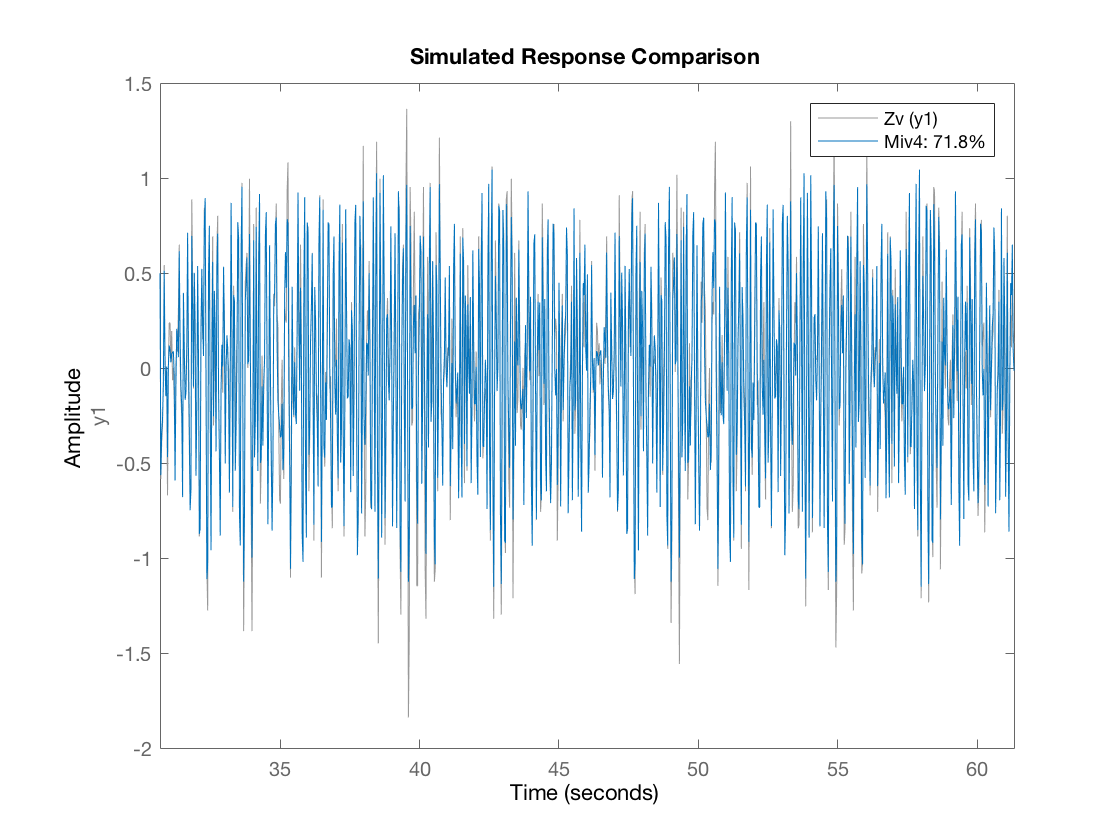
\includegraphics[height=5.5cm]{figures/c_iv4.png}
		\subcaption{Comparison of the output of the Instrumental Variables method model with the validation data $Zv$}\label{fig:c_iv4}
	\end{subfigure}
	\begin{subfigure}{.49\textwidth}
		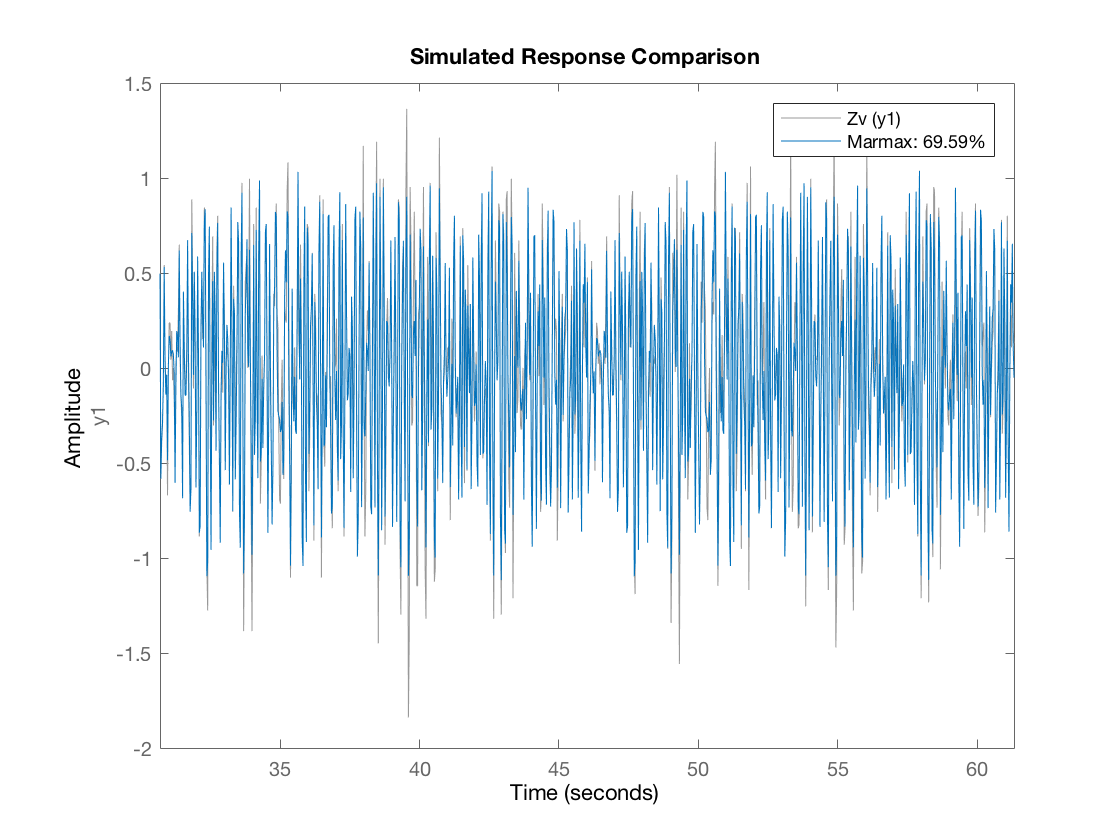
\includegraphics[height=5.5cm]{figures/c_armax.png}
		\subcaption{Comparison of the output of the ARMAX model with the validation data $Zv$}\label{fig:c_armax}
	\end{subfigure}\hfill
	\begin{subfigure}{.49\textwidth}
		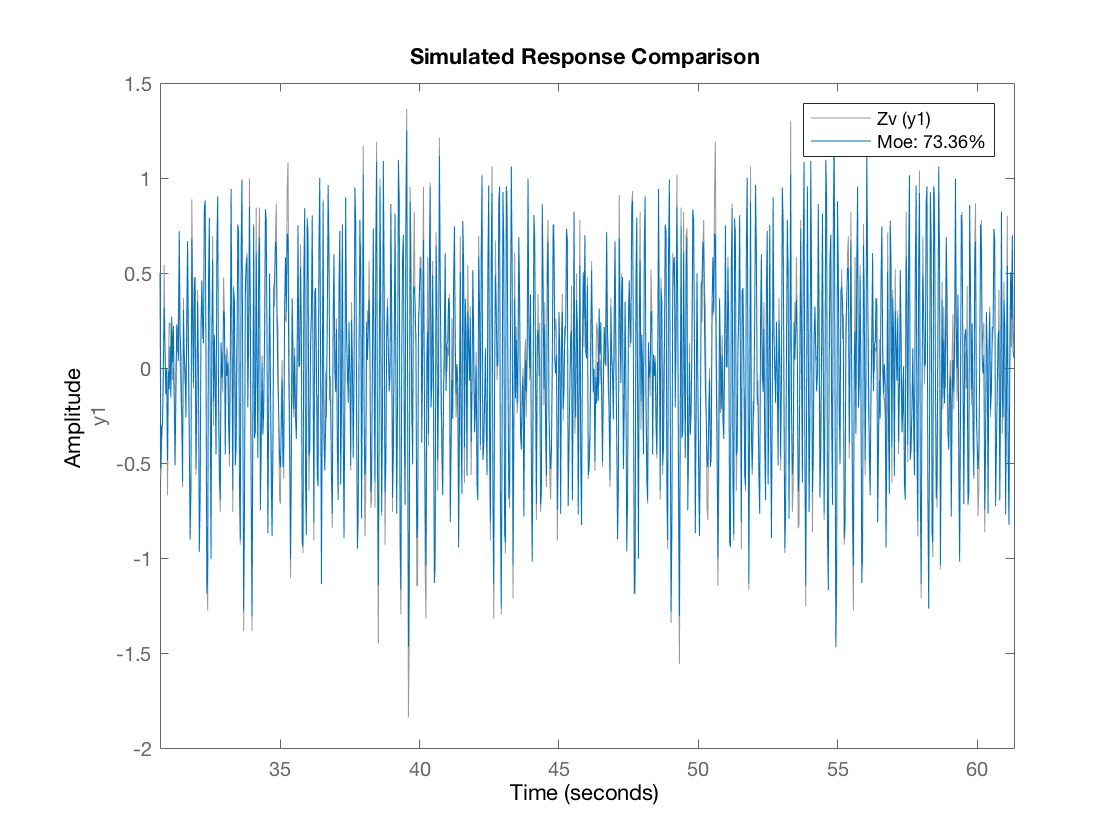
\includegraphics[height=5.5cm]{figures/c_oe.png}
		\subcaption{Comparison of the output of the Output Error model with the validation data $Zv$}\label{fig:c_oe}
	\end{subfigure}
	\begin{subfigure}{.49\textwidth}
		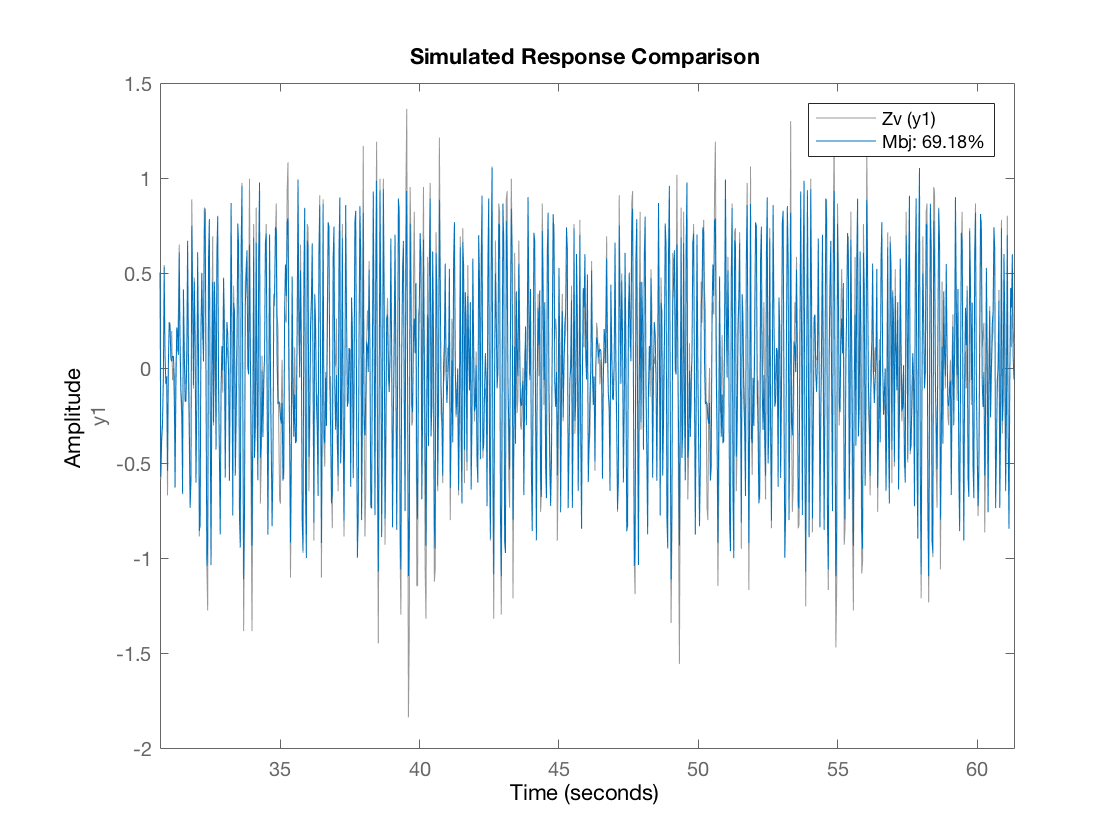
\includegraphics[height=5.5cm]{figures/c_bj.png}
		\subcaption{Comparison of the output of the Box Jenkins model with the validation data $Zv$}\label{fig:c_bj}
	\end{subfigure}\hfill
	\begin{subfigure}{.49\textwidth}
		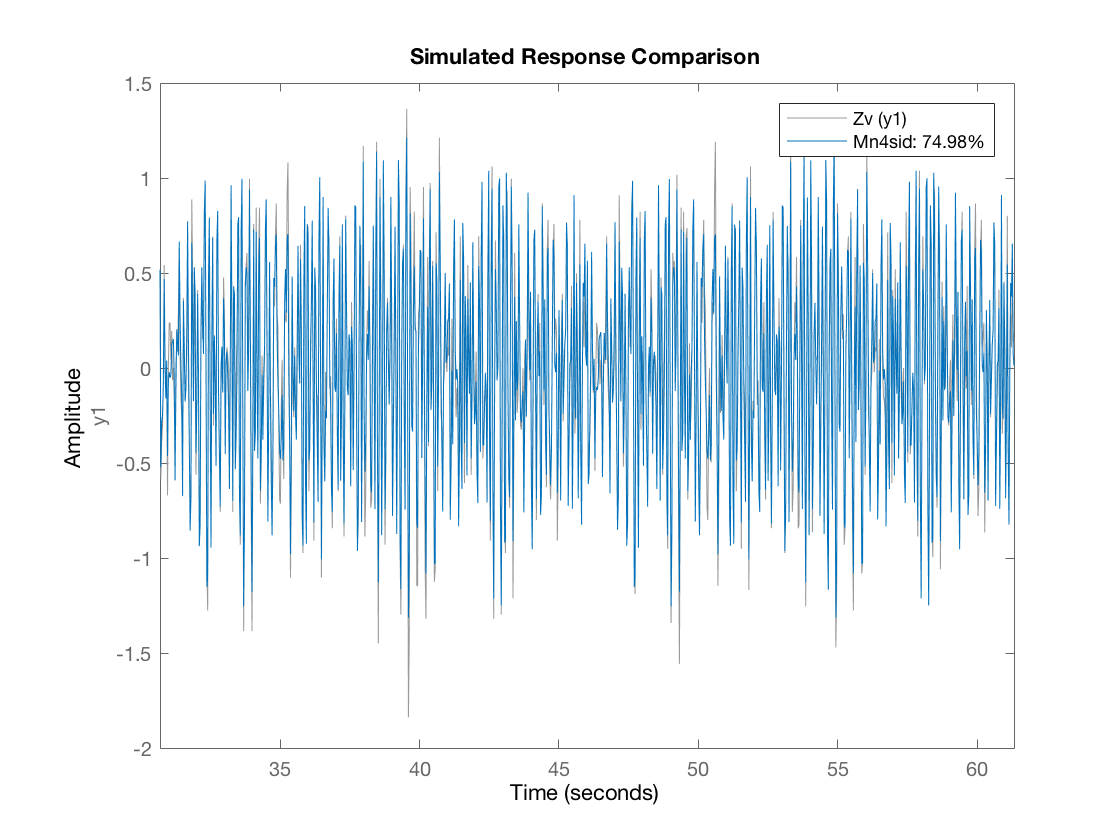
\includegraphics[height=5.5cm]{figures/c_n4sid.png}
		\subcaption{Comparison of the output of the State Space model with the validation data $Zv$}\label{fig:c_n4sid}
	\end{subfigure}
	\caption{Comparison of the measured output with the output of the models with the same input each time. The MATLAB command \texttt{compare} is used. }\label{fig:comparison}
\end{figure}

\paragraph{Frequency-Domain Validation: } Figure~\ref{fig:comparison_freq}.

\begin{figure}[h]
	\centering
	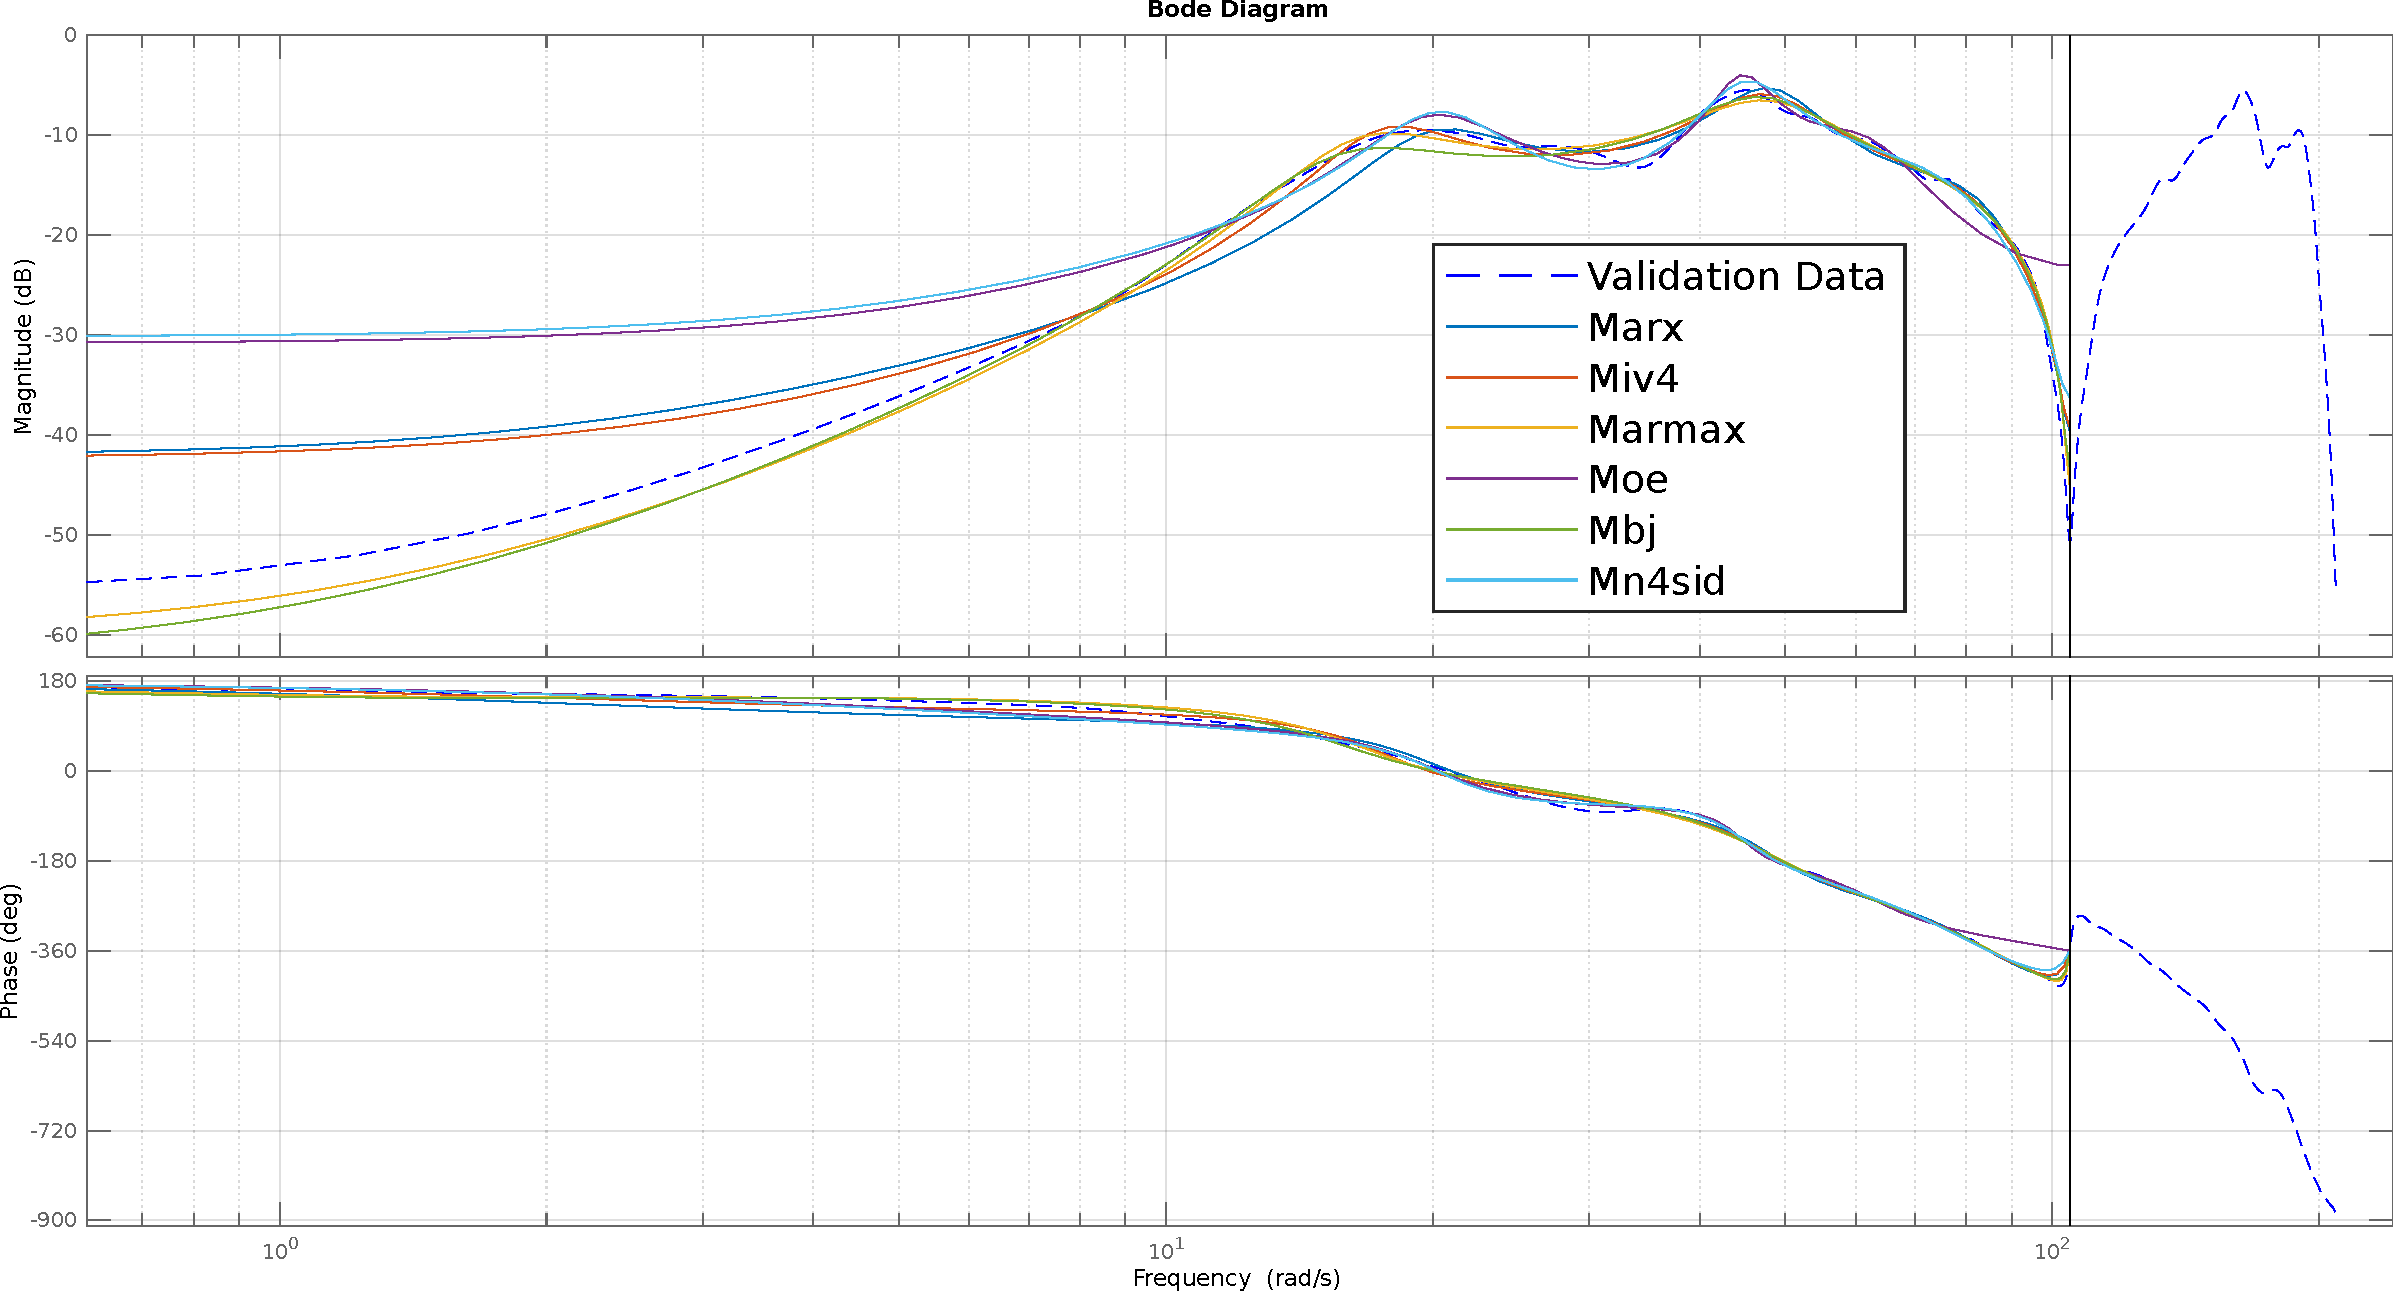
\includegraphics[width=\textwidth]{figures/bode_parametric.pdf}
	\caption{Comparison of the frequency response of the identified model and the frequency response of the validation data obtained using the spectral analysis method.}
	\label{fig:comparison_freq}
\end{figure}

\paragraph{Whiteness and Cross-Correlation Test: }
Afterwards, we want to validate our models by the whiteness test of the residuals $\epsilon$ and the cross-correlation of the residuals and the past inputs $u$.

\begin{itemize}
	\item Cross-correlation test: If the plant model is correctly identified, there is no information from the past inputs in the residuals and therefore, the residuals should be uncorrelated with those inputs. 
	For the cross-correlation test, an estimate of the cross-correlation between the residual and the input signal $\hat{R}_{\epsilon u}(h)$ is computed. The cross-correlation should be zero in order to validate the model. In practice, a statistical test with a $95\%$ confidence interval is used, where the values for the cross-correlation must lie within. This test can be used to validate the plant model for all structures. However, it gives no information about the validation of the noise model. 
	The results of the cross-correlation tests can be seen in the right part of Figures~\ref{fig:v_arx} to \ref{fig:v_n4sid}. 
	\item Whiteness test: For the models with a noise model (ARX, ARMAX and Box-Jenkins) we assume that the system noise is a white noise filtered by some transfer function. Therefore, if the parameters of the plant model and those of the noise model are correctly identified, the residual $\epsilon (k, \hat{\theta}) = y(k) - \hat{y}(k, \hat{\theta})$ will be white.
	The whiteness test checks the whiteness of the residual by computing the autocorrelation of $\epsilon$. This autocorrelation function will be zero for all $h \neq 0$, if $\epsilon$ is white. In practice, again a $95\%$ confidence interval is used, where the values for the cross-correlation must lie within.
	Therefore, this test is only reasonable for structures with a noise model.
	The results of the whiteness tests can be seen in the left part of Figures~\ref{fig:v_arx} to \ref{fig:v_n4sid}. 
\end{itemize}

\begin{figure}[h]
	\centering
	\begin{subfigure}{.49\textwidth}
		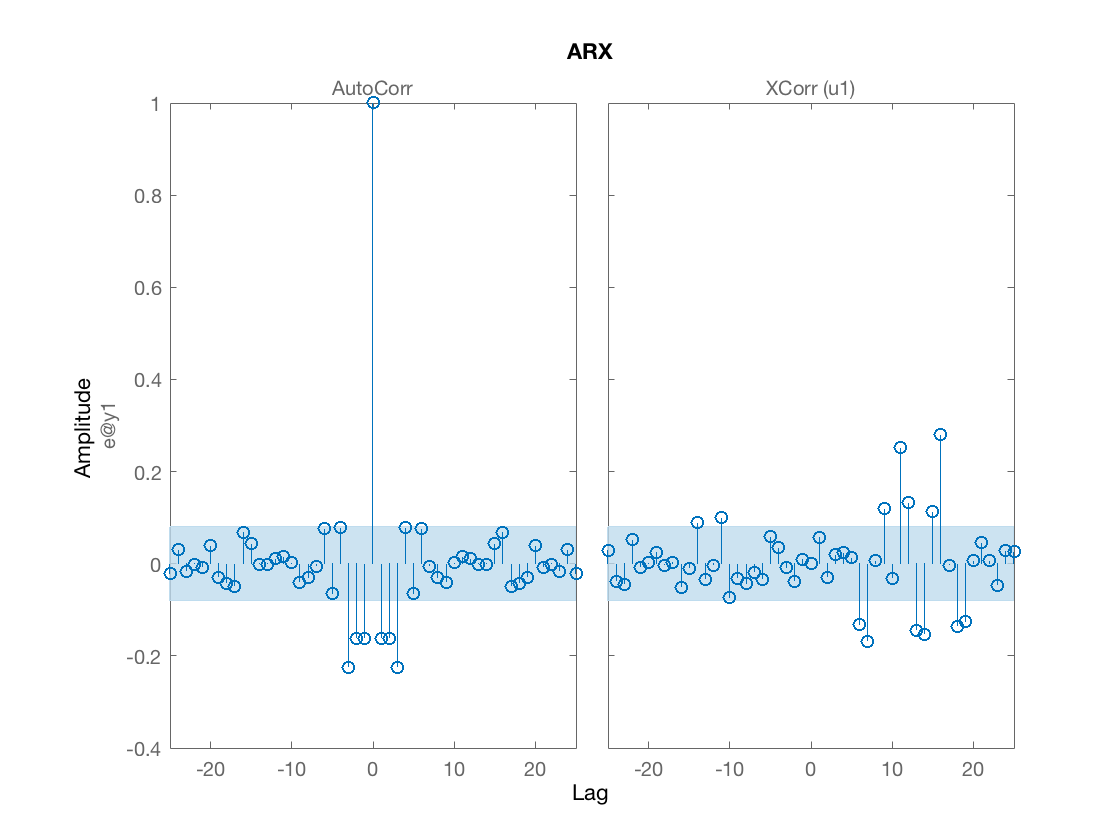
\includegraphics[height=5.5cm]{figures/v_arx.png}
		\subcaption{Whiteness test and cross-correlation test of the ARX model}\label{fig:v_arx}
	\end{subfigure}\hfill
	\begin{subfigure}{.49\textwidth}
		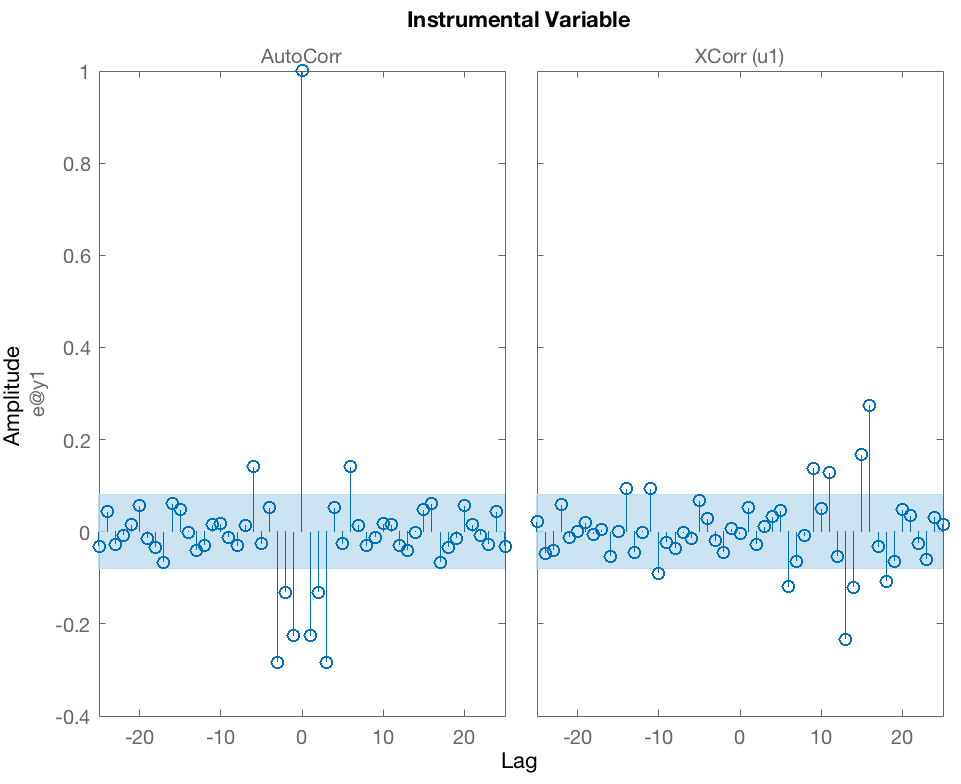
\includegraphics[height=5.5cm]{figures/v_iv.png}
		\subcaption{Whiteness test and cross-correlation test of the Instrumental Variables method}\label{fig:v_iv4}
	\end{subfigure}
	\begin{subfigure}{.49\textwidth}
		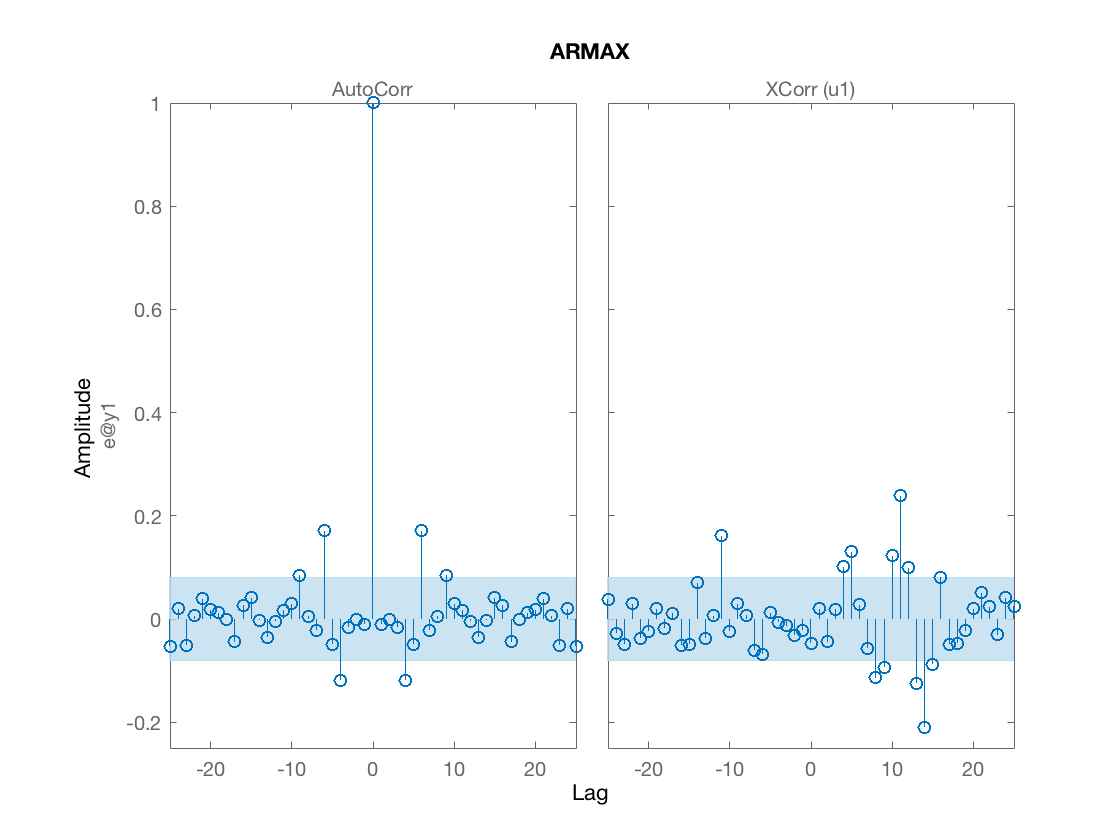
\includegraphics[height=5.5cm]{figures/v_armax.png}
		\subcaption{Whiteness test and cross-correlation test of the ARMAX model}\label{fig:v_armax}
	\end{subfigure}\hfill
	\begin{subfigure}{.49\textwidth}
		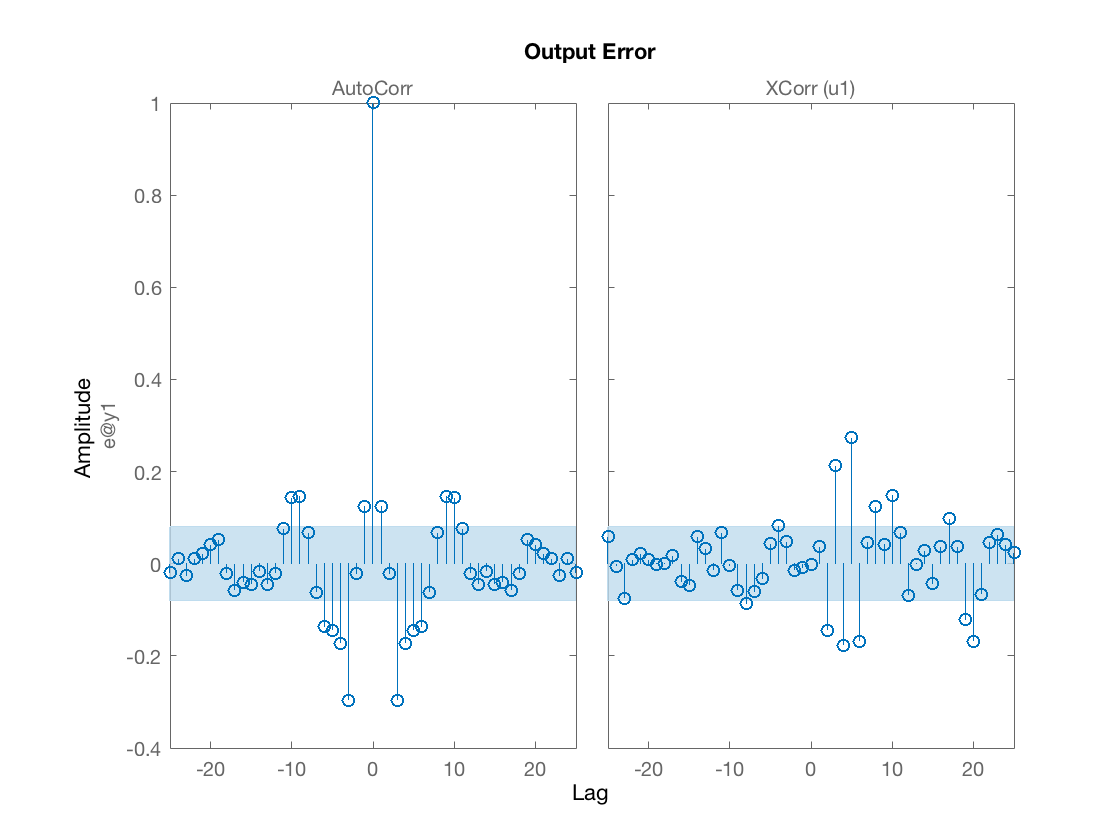
\includegraphics[height=5.5cm]{figures/v_oe.png}
		\subcaption{Whiteness test and cross-correlation test of the Output Error model}\label{fig:v_oe}
	\end{subfigure}
	\begin{subfigure}{.49\textwidth}
		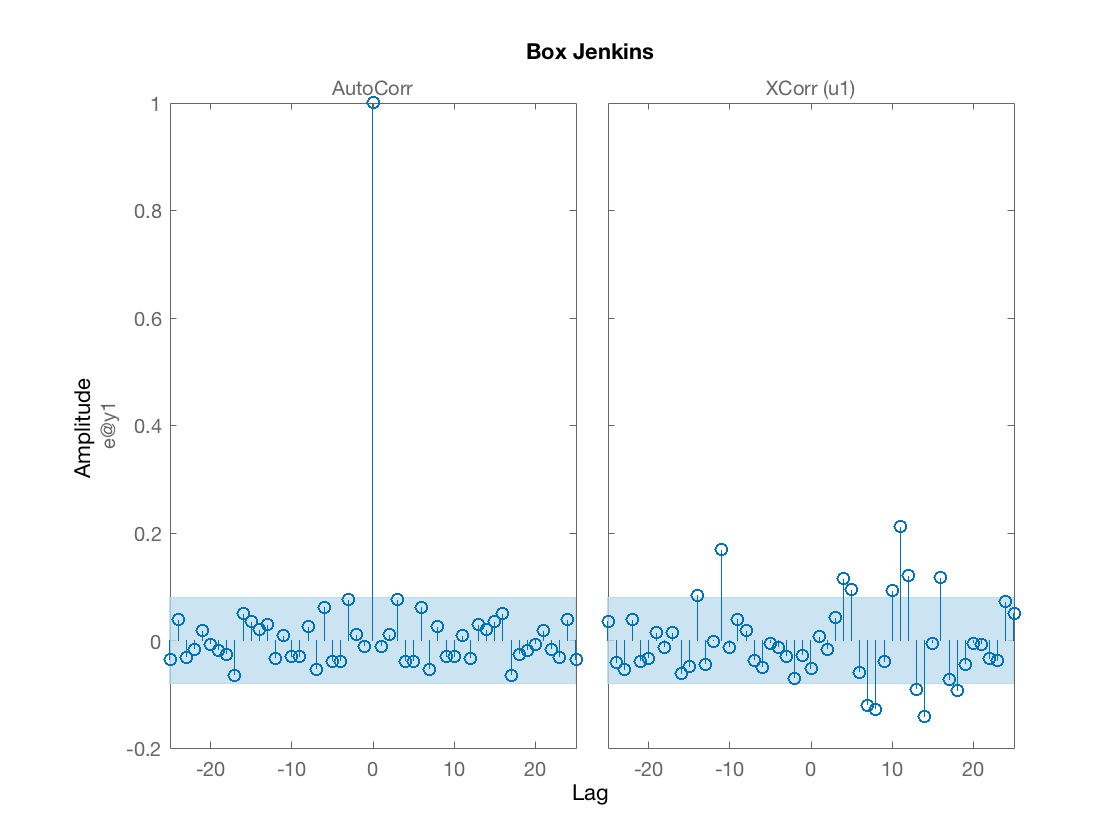
\includegraphics[height=5.5cm]{figures/v_bj.png}
		\subcaption{Whiteness test and cross-correlation test of the Box Jenkins model}\label{fig:v_bj}
	\end{subfigure}\hfill
	\begin{subfigure}{.49\textwidth}
		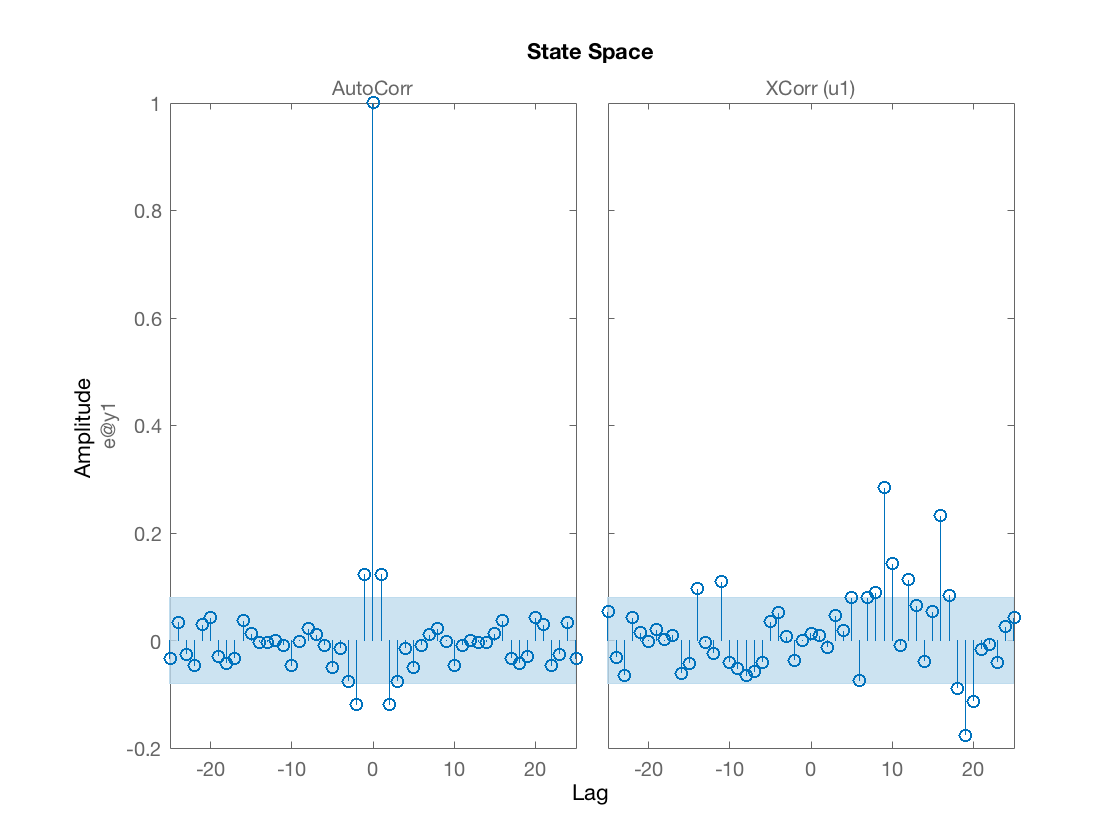
\includegraphics[height=5.5cm]{figures/v_ss.png}
		\subcaption{Whiteness test and cross-correlation test of the State Space model}\label{fig:v_n4sid}
	\end{subfigure}
	\caption{Whiteness test of the residuals and cross-correlation of the residuals and past inputs of different models with the MATLAB command \texttt{resid}.}
	\label{fig:test}
\end{figure}

Based on the results of the statistical tests of the identified models, we discuss about their validation below.
\begin{itemize}
\item{ARX model}
\item{Instrumental variables}
\item{ARMAX model}
\item{Output error structure} For the output error structure the whiteness test (left part of Figure~\ref{fig:v_oe}) can be ignored, as this structure does not include a noise model. However, the condition of the cross-correlation test is not met as there are several values of the cross-correlation function lying outside the confidence interval (right part in Figure~\ref{fig:v_oe}). This is why the output error structure is no validated model. 
\item{Box Jenkins} For the Box Jenkins model the residual is white as all values of the autocorrelation function $R_{\epsilon \epsilon}$ are within the confidence interval (left part of Figure~\ref{fig:v_bj}). Nevertheless, this model is not validated in the cross-correlation test, as several values of the cross-correlation function are bigger than the confidence interval (right part in Figure~\ref{fig:v_bj}).
\item{State space model}
Like for the output error structure, the whiteness test (left part of Figure~\ref{fig:v_n4sid}) does not make sense for the state space model, as this structure does not include a noise model. However, the cross-correlation test is not validated as there are several values of the cross-correlation function lying outside the confidence interval (right part in Figure~\ref{fig:v_n4sid}). This is why the state space model is not a validated model.
\end{itemize}




\appendix
\section{MATLAB Code}
\matlabcode{../matlab/ce2/FIR_model_identification.m}{Computing the finite impulse response of the system}{lst:FIR}
\matlabcode{../matlab/ce2/ARX_model_identification.m}{Matlab function for the ARX model identification technique including the instrumental variables method. Setting the iterations parameter to 1 will compute the plain ARX model without instrumental variables. A value greater than one uses IV to obtain asymptotically unbiased results.}{lst:ARX}
\matlabcode{../matlab/ce2/ss_identification.m}{State space identification using the subspace projection method.}{lst:ss_id}
\matlabcode{../matlab/ce2/estimate_delay.m}{Matlab function for the estimation of the delay using a FIR model.}{lst:delay}
\matlabcode{../matlab/ce2/parametric_identification.m}{Code for partitioning the data and creating the models}{lst:parametric}

\end{document}
